\documentclass[11pt,a4paper]{article}
\usepackage[left=25mm,right=25mm,top=25mm,bottom=25mm,headheight=15pt]{geometry}
\usepackage{amsmath,amsthm}
\usepackage{microtype}
\usepackage{unicode-math}
\setmainfont{lmroman10-regular.otf}[BoldFont=lmroman10-bold.otf,ItalicFont=lmroman10-italic.otf,BoldItalicFont=lmroman10-bolditalic.otf]
\setsansfont{lmsans10-regular.otf}[BoldFont=lmsans10-bold.otf,ItalicFont=lmsans10-oblique.otf]
\setmonofont{lmmono10-regular.otf}
\setmathfont{latinmodern-math.otf}
\usepackage{booktabs,array,tabularx,longtable}
\usepackage{placeins}
\usepackage{xcolor}
\definecolor{inkblue}{HTML}{203B50}
\usepackage{enumitem}
\usepackage{fancyhdr,lastpage}
\usepackage{tikz}
\usepackage{pgfplots}
\pgfplotsset{compat=1.18}
\usepackage{fancyvrb}
\newfontfamily\leanfont{DejaVuSansMono.ttf}[Scale=0.78]
\usepackage{hyperref}
\usepackage{bookmark}
\hypersetup{colorlinks=true,linkcolor=inkblue,citecolor=inkblue,urlcolor=inkblue,
  pdftitle={Counterexamples to the Robin spectral gap conjecture in every dimension},
  pdfauthor={Shurui Zheng},pdfsubject={Robin Laplacian, thin domains, spectral gap, convex domains, formal verification},
  pdflang={en-US}}
\pagestyle{fancy}
\fancyhf{}
\fancyhead[L]{\small Robin spectral gaps and effective end conditions}
\fancyhead[R]{}
\fancyfoot[C]{\small \thepage}
\renewcommand{\headrulewidth}{0pt}
\setlength{\parskip}{0.22em}
\linespread{1.04}
\setlength{\emergencystretch}{2em}
\widowpenalty=10000
\clubpenalty=10000
\allowdisplaybreaks[2]
\numberwithin{equation}{section}
\newtheoremstyle{paperplain}{8pt}{8pt}{\itshape}{}{\bfseries}{.}{.6em}{}
\theoremstyle{paperplain}
\newtheorem{theorem}{Theorem}[section]
\newtheorem{lemma}[theorem]{Lemma}
\newtheorem{proposition}[theorem]{Proposition}
\newtheorem{corollary}[theorem]{Corollary}
\newtheorem{conjecture}[theorem]{Conjecture}
\newtheorem{definition}[theorem]{Definition}
\theoremstyle{remark}
\newtheorem{remark}[theorem]{Remark}
\newcommand{\R}{\mathbb{R}}
\newcommand{\C}{\mathcal{C}}
\newcommand{\B}{\mathcal{B}}
\newcommand{\HH}{\mathcal{H}}
\newcommand{\dd}{\,\mathrm d}
\newcommand{\Tr}{\operatorname{Tr}}
\newcommand{\diam}{\operatorname{diam}}
\newcommand{\dist}{\operatorname{dist}}
\newcommand{\norm}[1]{\left\lVert#1\right\rVert}
\newcommand{\abs}[1]{\left\lvert#1\right\rvert}
\newcommand{\ip}[2]{\left\langle#1,#2\right\rangle}
\newcommand{\lean}[1]{\texttt{#1}}
\setlist[enumerate]{leftmargin=2em,itemsep=.35em,topsep=.4em}

\newcommand{\leancommit}{\texttt{8d24a660\allowbreak 8a4af7f2\allowbreak 1ae5fcf5\allowbreak 5f0e2ada\allowbreak ad3a86f6}}
\newcommand{\leanversion}{Lean~4.26.0}
\newcommand{\mathlibversion}{mathlib v4.26.0}
\newcommand{\leanfiles}{241}
\newcommand{\leanlines}{109{,}000}
\newcommand{\leanaxiomchecks}{379}
\newcommand{\leangeneralname}{\lean{mainTheorem\_general\_top}}

\title{Counterexamples to the Robin spectral gap conjecture in every dimension}
\author{Shurui Zheng\\[.6em]
  {\small Qiuzhen College, Tsinghua University, Beijing, China}\\[.3em]
  {\small \texttt{zhengsr23@mails.tsinghua.edu.cn}}}
\date{16 November 2026}

\begin{document}
\maketitle
\thispagestyle{plain}

\begin{abstract}
Andrews, Clutterbuck and Hauer conjectured that for $\alpha>0$ the gap
$\lambda_2-\lambda_1$ between the first two Robin eigenvalues of a bounded
convex domain in $\R^n$ is larger than the corresponding gap of an interval
of the same diameter. We show that this fails for every $n\ge2$ and every
$\alpha>0$. The counterexamples are thin capsules, the $R$-neighbourhoods of
a segment. As $R\to0$, the gap of the capsule of diameter $D$ converges to
the gap of the interval $(0,D)$ with Robin coefficient
$\beta_0=\alpha\,\omega_n/(2\omega_{n-1})$ in place of $\alpha$, where
$\omega_k$ is the volume of the unit ball of $\R^k$. Since $\beta_0<\alpha$
and the interval gap increases with the coefficient, the capsule gap lies
below the conjectured bound for all small $R$. The capsule is a special case
of a reduction theorem: on a thin cylinder of radius $R$ closed by convex
end caps of revolution, the low Robin eigenvalues, shifted by the transverse
ground-state energy, differ by $O(R)$ from those of an interval whose
endpoint coefficients depend only on the surface area and the volume of the
caps, and among all such caps the hemisphere gives the smallest coefficient.
The counterexample, the general reduction theorem, and the sharp cap
inequality are formally verified in Lean~4 with mathlib.
\end{abstract}

\noindent\textit{2020 Mathematics Subject Classification.} 35P15 (primary);
35J25, 35B25, 49R05, 68V20.\\
\textit{Keywords.} Robin Laplacian; spectral gap; convex domains; thin
domains; effective boundary conditions; formal verification.

\section{Introduction}\label{sec:intro}

\subsection{The Robin gap conjecture}
Let $\Omega\subset\R^n$ be a bounded convex domain and $\alpha\in\R$. The
Robin eigenvalue problem is
\[
 -\Delta u=\lambda u\ \text{ in }\Omega,\qquad
 \partial_\nu u+\alpha u=0\ \text{ on }\partial\Omega,
\]
with $\nu$ the outward unit normal. Its spectrum is discrete,
$\lambda_1(\Omega;\alpha)<\lambda_2(\Omega;\alpha)\le\cdots\to\infty$, with
$\lambda_j$ counted with multiplicity and understood in the variational
sense of Section~\ref{sec:setup}; the case $\alpha=0$ is the Neumann
problem and $\alpha=\infty$ the Dirichlet problem. The \emph{spectral gap} $\lambda_2-\lambda_1$ controls, for instance,
the rate of convergence to equilibrium of the associated diffusion
\cite{Smits}. At both ends of the parameter range the sharp bound for the gap under a
diameter constraint is classical. For Neumann conditions it is the
Payne--Weinberger inequality $\lambda_2\ge\pi^2/D^2$ \cite{PW,Bebendorf}.
For Dirichlet conditions it is the fundamental gap theorem
$\lambda_2-\lambda_1\ge3\pi^2/D^2$ of Andrews and Clutterbuck \cite{AC},
conjectured by van den Berg \cite{vandenBerg}, Ashbaugh and Benguria
\cite{AshbaughBenguria}, and Yau \cite{Yau}. In both cases the constant is
the gap of the interval $(0,D)$ with the same boundary condition, and it is
approached by thin neighbourhoods of a segment. Andrews, Clutterbuck and Hauer conjectured that the same holds
throughout the Robin range \cite[Section~10]{ACH}; in the form recorded by
Laugesen \cite[Conjecture~F]{Laugesen} the conjecture reads as follows.

\begin{conjecture}[Robin gap conjecture]\label{conj:gap}
Fix $\alpha>0$ and $n\ge2$. Every bounded convex domain $\Omega\subset\R^n$
of diameter $D$ satisfies
\begin{equation}\label{eq:conjecture}
 \lambda_2(\Omega;\alpha)-\lambda_1(\Omega;\alpha)
 >\lambda_2((0,D);\alpha)-\lambda_1((0,D);\alpha).
\end{equation}
\end{conjecture}

Other versions allow equality and $\alpha\ge0$ \cite{Kielty}, or add a convex
potential \cite[Section~10]{ACH}. The conjecture is known for rectangular
boxes, for every $\alpha\in\R$ \cite[Theorem~3.8]{Laugesen}, and in one
dimension sharp gap bounds are known for Schr\"odinger operators with
convex or single-well potentials, for Dirichlet \cite{Lavine} and for
Robin conditions \cite{ACH1D,AshbaughKielty}. Andrews,
Clutterbuck and Hauer proved the weaker bound $\pi^2/D^2$ under the
additional assumption that the Robin ground state is log-concave
\cite[Theorem~2.1]{ACH}, and showed that log-concavity fails on some convex
domains for small $\alpha$ \cite[Theorem~1.2]{ACH}; log-concavity does hold
on uniformly convex $C^{3,1}$ domains when $\alpha$ is large
\cite{YeZhang}. For $\alpha<0$ the analogue of
\eqref{eq:conjecture} is false: Kielty \cite{Kielty} showed that thin double
cones have exponentially small gap, because for $\alpha<0$ the eigenfunctions
localize at the vertices. For positive parameters, Colbrook
\cite{Colbrook} has presented a three-dimensional counterexample using a
different thin-domain mechanism; we discuss its relation to the present
results below. Our construction works in every dimension $n\ge2$, including
the plane, and yields a quantitative reduction theorem with explicit
effective endpoint coefficients. For a related conjecture of Laugesen,
that the ratio $\lambda_2/\lambda_1$ decreases in $\alpha$, counterexamples
were recently given by Dai and Sun \cite{DaiSun}.

\subsection{The counterexample}
Write $m=n-1$, let $|\cdot|$ denote Lebesgue measure and $\HH^k$ the
$k$-dimensional Hausdorff measure, and let $\omega_k=|B_k(1)|$ be the
volume of the unit ball of $\R^k$. For $p,q,\ell>0$ let $\mu_1(p,q;\ell)<\mu_2(p,q;\ell)<\cdots$ be the
eigenvalues of $-f''$ on $(0,\ell)$ with the Robin conditions $f'(0)=pf(0)$
and $f'(\ell)=-qf(\ell)$, and let
\begin{equation}\label{eq:G-intro}
 G_\beta(\ell)=\mu_2(\beta,\beta;\ell)-\mu_1(\beta,\beta;\ell)
\end{equation}
be the gap of the interval with coefficient $\beta$ at both ends; the
right-hand side of \eqref{eq:conjecture} is $G_\alpha(D)$. For $L>0$ and
$0<R<L/2$ let $S_R$ be a segment of length $L-2R$ and
\[
 \Omega_R=\{P\in\R^n:\ \dist(P,S_R)<R\}
\]
the \emph{capsule} around it: a cylinder of radius $R$ closed by two
hemispheres. It is convex and of class $C^{1,1}$.

\begin{theorem}\label{thm:intro-counter}
Let $n\ge2$, $\alpha>0$, $L>0$, and $\beta_0=\alpha\,\omega_n/(2\omega_{n-1})$.
Then $0<\beta_0<\alpha$, $\diam\Omega_R=L$, and
\begin{equation}\label{eq:capsule-limit}
 \lambda_2(\Omega_R;\alpha)-\lambda_1(\Omega_R;\alpha)
 =G_{\beta_0}(L)+O(R)\qquad(R\downarrow0).
\end{equation}
In particular, there is $R_*>0$ such that
\begin{equation}\label{eq:capsule-strict}
 \lambda_2(\Omega_R;\alpha)-\lambda_1(\Omega_R;\alpha)
 \le\tfrac12\bigl(G_\alpha(L)+G_{\beta_0}(L)\bigr)
 <G_\alpha(\diam\Omega_R)\qquad(0<R<R_*).
\end{equation}
\end{theorem}

The point of \eqref{eq:capsule-limit} is that the limiting Robin coefficient
is $\beta_0$ rather than $\alpha$. The interval gap $G_\beta(L)$ is strictly
increasing in $\beta$ \cite{Smits} (Proposition~\ref{prop:gap-monotone}),
so the margin $G_\alpha(L)-G_{\beta_0}(L)$ in \eqref{eq:capsule-strict} is
positive; it depends only on $n$, $\alpha$ and $L$, not on $R$. In low
dimensions
\[
 \frac{\beta_0}{\alpha}=\frac\pi4,\ \frac23,\ \frac{3\pi}{16},\ \frac8{15}
 \qquad(n=2,3,4,5),
\]
and for $\alpha=4$, $L=1$ the limiting gaps are $15.21$ for $n=2$ and
$14.53$ for $n=3$, against the conjectured lower bound $G_4(1)=16.32$
(Figure~\ref{fig:gap}); they lie about $7\%$ and $11\%$ below the bound,
respectively. A finite element computation (Section~\ref{sec:numerics})
shows that the capsule gap drops below $G_\alpha(L)$ at $R\approx0.09$ in
both cases. Since the inequality in \eqref{eq:capsule-strict} is strict,
the capsules also violate the non-strict version of the conjecture, its
extension to $\alpha\ge0$ \cite{Kielty}, and, with zero potential, the
version with a convex potential \cite[Section~10]{ACH}.

\begin{figure}[t]
\centering
\begin{tikzpicture}
\begin{axis}[
  width=0.72\textwidth, height=0.42\textwidth,
  xmin=0, xmax=12, ymin=8.5, ymax=31,
  xlabel={$\beta$}, ylabel={$G_\beta(1)$},
  axis lines=left, tick label style={font=\small},
  label style={font=\small}, clip=false]
  \addplot[thick,blue!70!black] table {gapcurve.dat};
  \addplot[dashed,gray,domain=0:12] {pi^2};
  \addplot[dashed,gray,domain=0:12] {3*pi^2};
  \node[anchor=south east,font=\scriptsize,gray] at (axis cs:12,9.87) {Neumann $\pi^2$};
  \node[anchor=north east,font=\scriptsize,gray] at (axis cs:12,29.61) {Dirichlet $3\pi^2$};
  \addplot[only marks,mark=*,mark size=1.6pt] coordinates {(4,16.3182)};
  \addplot[only marks,mark=o,mark size=1.8pt] coordinates {(3.14159,15.2064) (2.66667,14.5302)};
  \draw[gray] (axis cs:4,16.3182) -- (axis cs:6.2,14.2) node[anchor=west,font=\scriptsize,black] {$\beta=\alpha$: flat ends};
  \draw[gray] (axis cs:3.14159,15.2064) -- (axis cs:5.2,12.6) node[anchor=west,font=\scriptsize,black] {$\beta_0$, capsule, $n=2$};
  \draw[gray] (axis cs:2.66667,14.5302) -- (axis cs:4.2,11.1) node[anchor=west,font=\scriptsize,black] {$\beta_0$, capsule, $n=3$};
\end{axis}
\end{tikzpicture}
\caption{The interval gap $G_\beta(1)=\mu_2(\beta,\beta;1)-\mu_1(\beta,\beta;1)$
as a function of the Robin coefficient $\beta$, increasing from the Neumann
value $\pi^2$ to the Dirichlet value $3\pi^2$. For $\alpha=4$ the filled
point is the gap $G_\alpha(1)$ of the conjecture, the open points are the
limiting capsule gaps $G_{\beta_0}(1)$ for $n=2$
($\beta_0=\pi\alpha/4$) and $n=3$ ($\beta_0=2\alpha/3$).
By scaling, $G_\beta(L)=L^{-2}G_{L\beta}(1)$.}\label{fig:gap}
\end{figure}

\subsection{Effective Robin conditions at the ends}
Theorem~\ref{thm:intro-counter} is a special case of a reduction theorem
for thin capped cylinders (Theorem~\ref{thm:intro-main}), and $\beta_0$ is
the minimum in a sharp geometric inequality for the caps
(Theorem~\ref{thm:intro-cap}).

A single trial function already suggests \eqref{eq:capsule-limit}. Let
$\nu_R=\lambda_1(B_m(R);\alpha)$ be the first Robin eigenvalue of the
cross-section and $\psi_R$ its eigenfunction, normalized in $L^2(B_m(R))$.
When $\alpha R$ is small, $\psi_R\approx(\omega_mR^m)^{-1/2}$ and
$\nu_R\approx m\alpha/R$, the lateral Robin energy per unit volume of the
cylinder. Take $u(x,y)=F(x)\psi_R(y)$ in the cylindrical part and extend
$u$ into each cap by its value on the interface disk. After subtracting
$\nu_R$ times the mass, the cylinder contributes $\int|F'|^2$. A cap $\C$ of volume $R^n|\C|$, whose boundary outside the interface disk
we call $\Gamma$, has exposed surface area $R^m\HH^m(\Gamma)$ and
contributes
the Robin term $\alpha\HH^m(\Gamma)|F|^2/\omega_m$ and the subtracted volume
term $-\nu_RR|\C|\,|F|^2/\omega_m\approx-m\alpha|\C|\,|F|^2/\omega_m$ at the
corresponding endpoint. The subtraction of $\nu_R$ thus credits every unit
of cap volume with the lateral Robin energy $m\alpha$ that a unit of
cylinder would pay, and only the excess surface $\HH^m(\Gamma)-m|\C|$
survives, as an endpoint Robin coefficient
\[
 \beta(\C)=\frac{\alpha}{\omega_m}\bigl(\HH^m(\Gamma)-m|\C|\bigr).
\]
A flat end has excess $\omega_m$ and $\beta=\alpha$; a hemisphere has
excess $\omega_{m+1}/2<\omega_m$ and $\beta=\beta_0$. Replacing the flat end
by a hemisphere weakens the effective boundary condition, and a weaker Robin
condition means a smaller gap.

To make this precise, an \emph{admissible end cap}
(Definition~\ref{def:cap}) is a convex solid of revolution
\[
 \C=\{(s,z)\in\R\times\R^m:\ -K<s<0,\ |z|<\theta(s)\}
\]
whose profile $\theta:(-K,0)\to(0,1]$ is concave and nonincreasing with
$\theta(-K^+)=1$. It meets the unit cylinder along the entrance disk
$\Sigma=\{-K\}\times B_m(1)$, and $\Gamma=\partial\C\setminus\overline\Sigma$
is its exposed boundary, including the terminal disk if $\theta(0^-)>0$
(Figure~\ref{fig:domain}). Given two such caps $\C_\pm$ of lengths $K_\pm$
and $L>0$, the \emph{thin domain} $\Omega_R$, $0<R<L/(K_-+K_+)$, is the
convex domain of axial span $L$ obtained from a cylinder of radius $R$ by
closing its ends with copies of $\C_\pm$ scaled by $R$
(Definition~\ref{def:domain}); the capsule is the case of two unit
hemispheres.

\begin{figure}[t]
\centering
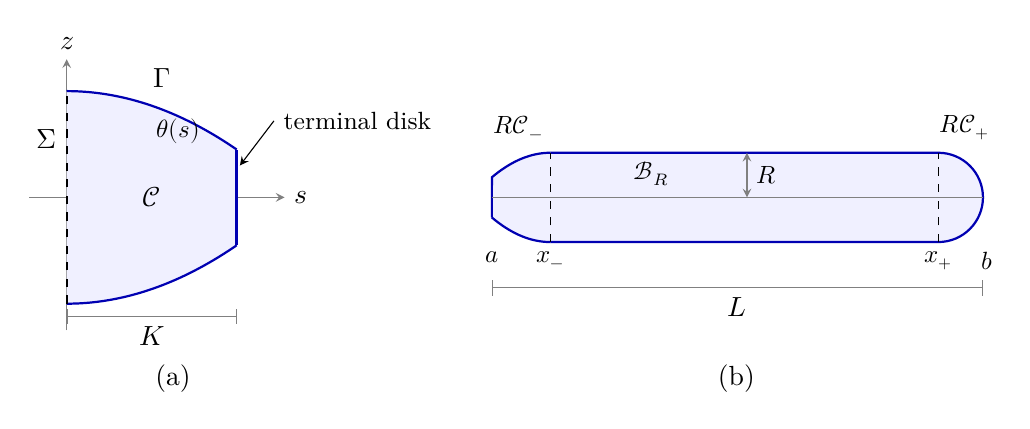
\begin{tikzpicture}[scale=1.35,>=stealth]
  \begin{scope}
    \def\K{1.6}
    \draw[->,gray] (-\K-0.35,0) -- (0.45,0) node[right,black] {$s$};
    \draw[->,gray] (-\K,-1.25) -- (-\K,1.3) node[above,black] {$z$};
    \fill[blue!6] plot[domain=-\K:0,samples=40] (\x,{1-0.55*((\x+\K)/\K)^2})
      -- (0,-0.45) -- plot[domain=0:-\K,samples=40] (\x,{-(1-0.55*((\x+\K)/\K)^2)}) -- cycle;
    \draw[thick,blue!70!black] plot[domain=-\K:0,samples=40] (\x,{1-0.55*((\x+\K)/\K)^2});
    \draw[thick,blue!70!black] plot[domain=-\K:0,samples=40] (\x,{-(1-0.55*((\x+\K)/\K)^2)});
    \draw[very thick,blue!70!black] (0,-0.45) -- (0,0.45);
    \draw[dashed,thick] (-\K,-1) -- (-\K,1);
    \node[left] at (-\K,0.55) {$\Sigma$};
    \node at (-0.7,1.12) {$\Gamma$};
    \node at (-0.8,0) {$\C$};
    \draw[->] (0.35,0.72) node[right,font=\small] {terminal disk} -- (0.03,0.3);
    \draw[|-|,gray] (-\K,-1.12) -- (0,-1.12) node[midway,below,black] {$K$};
    \node[font=\small] at (-0.55,0.62) {$\theta(s)$};
    \node at (-0.6,-1.7) {(a)};
  \end{scope}
  \begin{scope}[xshift=2.4cm]
    \def\R{0.42}
    \fill[blue!6] (0.55,\R) -- (4.2,\R) arc (90:-90:\R) -- (0.55,-\R)
      -- plot[domain=0.55:0,samples=30] (\x,{-\R*(1-0.55*((0.55-\x)/0.55)^2)})
      -- (0,-0.45*\R) -- (0,0.45*\R)
      -- plot[domain=0:0.55,samples=30] (\x,{\R*(1-0.55*((0.55-\x)/0.55)^2)}) -- cycle;
    \draw[thick,blue!70!black] (0.55,\R) -- (4.2,\R) arc (90:-90:\R) -- (0.55,-\R);
    \draw[thick,blue!70!black] plot[domain=0.55:0,samples=30] (\x,{\R*(1-0.55*((0.55-\x)/0.55)^2)})
      -- (0,-0.45*\R) -- plot[domain=0:0.55,samples=30] (\x,{-\R*(1-0.55*((0.55-\x)/0.55)^2)});
    \draw[dashed] (0.55,-\R) -- (0.55,\R);
    \draw[dashed] (4.2,-\R) -- (4.2,\R);
    \draw[gray] (0,0) -- (4.62,0);
    \draw[|-|,gray] (0,-0.85) -- (4.62,-0.85) node[midway,below,black] {$L$};
    \node[below,font=\small] at (0,-0.42) {$a$};
    \node[below,font=\small] at (0.55,-0.42) {$x_-$};
    \node[below,font=\small] at (4.2,-0.42) {$x_+$};
    \node[below,font=\small] at (4.66,-0.42) {$b$};
    \draw[<->,gray] (2.4,0) -- (2.4,\R) node[midway,right,black,font=\small] {$R$};
    \node[font=\small] at (1.5,0.22) {$\B_R$};
    \node[above,font=\small] at (0.25,0.45) {$R\C_-$};
    \node[above,font=\small] at (4.45,0.45) {$R\C_+$};
    \node at (2.3,-1.7) {(b)};
  \end{scope}
\end{tikzpicture}
\caption{(a) An admissible end cap $\C$ with entrance disk $\Sigma$ and
exposed boundary $\Gamma$, which here contains a terminal disk.
(b) Axial section of the thin domain $\Omega_R$, in the notation of
Section~\ref{sec:setup}: a cylinder $\B_R$ of radius $R$, closed on the left
by a scaled copy of a cap with a terminal disk and on the right by a
hemisphere. The interfaces (dashed) carry no boundary condition. Schematic,
not to scale.}\label{fig:domain}
\end{figure}

\begin{theorem}\label{thm:intro-main}
Let $n\ge2$, $\alpha>0$, $L>0$, let $\C_-$, $\C_+$ be admissible end caps,
let $\Omega_R$ be the thin domain of Definition~\ref{def:domain}, and set
$\nu_R=\lambda_1(B_m(R);\alpha)$. For every $J\in\mathbb N$ there are
$C_J,R_J>0$ such that
\begin{equation}\label{eq:main}
 \bigl|\lambda_j(\Omega_R;\alpha)-\nu_R-\mu_j\bigl(\beta(\C_-),\beta(\C_+);L\bigr)\bigr|
 \le C_JR\qquad(1\le j\le J,\ 0<R<R_J).
\end{equation}
\end{theorem}

\begin{theorem}\label{thm:intro-cap}
Every admissible cap satisfies $\HH^m(\Gamma)-m|\C|\ge\omega_{m+1}/2$, that
is, $\beta(\C)\ge\beta_0$. Equality holds if and only if $K\ge1$ and $\C$ is
the unit hemisphere $\{|z|<\sqrt{1-(s+1)^2},\ -1<s<0\}$, extended at the
entrance by the cylinder $(-K,-1]\times B_m(1)$ when $K>1$.
\end{theorem}

Theorem~\ref{thm:intro-counter} follows by applying
Theorem~\ref{thm:intro-main} to two hemispheres with $J=2$ and using the
monotonicity of $G_\beta$ in $\beta$ (Section~\ref{sec:capsule}). By
Theorem~\ref{thm:intro-cap}, among thin cylinders closed by two identical
caps of revolution, hemispheres give the smallest limiting gap. The same
argument applies to every cap with $\beta(\C)<\alpha$, in particular to
caps arbitrarily close to a flat end (Section~\ref{sec:nearflat}): the
flat-ended cylinder, which realizes the conjectured bound in the limit, is
not a local minimizer of the limiting gap among thin capped cylinders.

\emph{Scheme of the proof of Theorem~\ref{thm:intro-main}.} The
trial-function computation is made rigorous uniformly on $J$-dimensional
spaces. In the cylinder we use an exact orthogonal decomposition with
respect to $\psi_R$, so that the bulk energy separates without error and
the transverse fluctuations are penalized at order $R^{-2}$
(Section~\ref{sec:transverse}). In each cap we rescale to the fixed domain
$\C$; the component along the transverse ground state contributes
$\beta(\C)|F|^2$ up to $O(R)$, and all other components are penalized at
order $R^{-1}$ (Section~\ref{sec:cap-lemma}). The lower bound then follows
from a finite-codimension min--max argument, the upper bound from a uniform
estimate on the trial space (Section~\ref{sec:proof}).

\emph{Scheme of the proof of Theorem~\ref{thm:intro-cap}.} The unit vector
field $X(s,z)=(\sqrt{1-|z|^2},z)$ has divergence $m$, and the divergence
theorem expresses the defect $\HH^m(\Gamma)-m|\C|-\omega_{m+1}/2$ as
$\int_\Gamma(1-X\cdot\nu)\dd\HH^m\ge0$. For a cap of revolution this is a
one-dimensional identity for the profile, which we prove directly
(Section~\ref{sec:calibration}).

\subsection{Related work}

Colbrook's manuscript \cite{Colbrook} constructs a thin three-dimensional
convex polytope whose transverse perimeter-to-area ratio produces two
wells separated by a barrier. Its gap tends to zero as the thickness
vanishes; a smoothing argument then gives a $C^\infty$ strictly convex
counterexample with $\alpha=1$. The manuscript is presented as a proposed
resolution pending independent mathematical review and does not claim
proof-assistant verification.

The present mechanism is an effective end condition rather than a
transverse double well. On capsules of fixed diameter, the gap converges
to the positive interval gap $G_{\beta_0}(L)$ with $\beta_0<\alpha$.
The results cover every $n\ge2$, in particular $n=2$, and also include
$O(R)$ asymptotics for general admissible end caps, a sharp cap inequality
with equality cases, and a Lean formalization. Our direct capsule examples
are $C^{1,1}$ and are not strictly convex; we do not claim here the smooth
strictly convex realization established in Colbrook's proposed construction.
The two constructions therefore address different geometric mechanisms
and give complementary spectral information.


Spectral asymptotics in thin domains and thin tubes have a long history; see
\cite{HaleRaugel,FriedlanderSolomyak,BorisovFreitas,Grieser} and the
references there, and \cite{BFK} for the Robin problem in general. For the
Robin Laplacian on collapsing domains, Pankrashkin and Vogel \cite{PankrashkinVogel}
obtained the eigenvalue asymptotics of sharp infinite cones with an
arbitrary cross-section $\omega$; the answer is governed by the ratio
$|\partial\omega|/|\omega|$, which plays the role of $m\alpha/R$ here.
Cacciapuoti and Finco \cite{CacciapuotiFinco} treat thin Robin waveguides
collapsing onto graphs. Closest to Theorem~\ref{thm:intro-main} is the work
of Bouchitt\'e, Mascarenhas and Trabucho \cite{BMT} on thin Robin
waveguides with flat bases. There the
lateral Robin coefficient is scaled like $\gamma/\varepsilon$, so the
transverse problem stays a genuine Robin problem at unit scale, and the flat
bases carry their own coefficients, which enter the limit through their
average against the transverse ground state. In our setting the Robin
parameter $\alpha$ is fixed, so the transverse problem is close to the
Neumann problem, the ends may be curved, and the endpoint coefficient is
produced by the geometry of the cap alone. Thin convex domains have been reduced to one-dimensional problems before,
notably by Grieser and Jerison \cite{GrieserJerison} for the Dirichlet
problem, and gap conjectures have been broken by thin domains: Bourni,
Clutterbuck, Nguyen, Stancu, Wei and Wheeler \cite{Bourni} showed that the
fundamental gap of convex domains in hyperbolic space can be arbitrarily
small.

Asymptotic analysis has produced counterexamples to Robin conjectures
before. Freitas and Krej\v{c}i\v{r}\'{\i}k \cite{FreitasKrejcirik} disproved
Bareket's conjecture on the first Robin eigenvalue with negative parameter
by an expansion in the parameter, and Dietze and Pankrashkin
\cite{DietzePankrashkin} settled a question of \cite{BFK} on the principal
eigenvalue for large negative parameters. In Kielty's counterexamples for
$\alpha<0$ \cite{Kielty} the eigenfunctions concentrate at the vertices of a
double cone and the gap collapses; here the eigenfunctions are, in the thin
limit, those of an interval problem whose boundary condition has been
weakened.

\subsection{Formal verification}
We give machine-checked proofs in Lean~4 \cite{Lean4}, using mathlib
\cite{mathlib}, of the counterexample, the reduction theorem, and the sharp
cap inequality.

The formalization covers Theorems~\ref{thm:intro-counter}--\ref{thm:intro-cap}
in their full stated generality, including every admissible pair of caps in
the reduction theorem and every dimension $n\ge2$.

The development includes the Sobolev and trace results needed for the
reduction and identifies the variational eigenvalues with those of the
self-adjoint Robin Laplacian. Appendix~\ref{sec:formal} presents the formal
definitions and theorem declarations.

\subsection{Organization}
Section~\ref{sec:setup} fixes the geometry and the conventions.
Section~\ref{sec:calibration} proves Theorem~\ref{thm:intro-cap} and
Section~\ref{sec:interval} collects facts about interval Robin problems.
Sections~\ref{sec:transverse}--\ref{sec:proof} prove
Theorem~\ref{thm:intro-main}. Section~\ref{sec:capsule} proves
Theorem~\ref{thm:intro-counter}, extends it to other end caps, and reports
a finite element computation. Section~\ref{sec:open} lists open questions,
and Appendix~\ref{sec:formal} describes the formal verification.

\section{Setting and conventions}\label{sec:setup}

\subsection{Robin forms and the interval problem}
All functions are real-valued and all Hilbert spaces are real. Let
$n\ge2$, $m=n-1$, $\alpha>0$ and $L>0$. For a bounded Lipschitz domain
$U\subset\R^N$, $N\ge1$, consider
\[
 q_U[u]=\int_U|\nabla u|^2\dd x+\alpha\int_{\partial U}|\Tr u|^2\dd\HH^{N-1},
 \qquad N_U[u]=\int_U|u|^2\dd x,\qquad u\in H^1(U),
\]
where $\Tr$ is the boundary trace; the associated boundary condition is
$\partial_\nu u+\alpha u=0$ with $\nu$ the outward unit normal. The Robin
eigenvalues are defined by the min--max principle,
\begin{equation}\label{eq:minmax}
 \lambda_j(U;\alpha)=
 \inf_{\substack{V\subset H^1(U)\\ \dim V=j}}
 \sup_{0\ne u\in V}\frac{q_U[u]}{N_U[u]},\qquad j\ge1,
\end{equation}
so that $\lambda_1(U;\alpha)\le\lambda_2(U;\alpha)\le\cdots$ with
multiplicity. For background on the Robin problem see \cite{BFK,Laugesen}.

On an interval of length $\ell$ and for $p,q>0$, the form
\begin{equation}\label{eq:interval-form}
 a_{p,q;\ell}[f]=\int_0^\ell |f'|^2\dd x+p|f(0)|^2+q|f(\ell)|^2
\end{equation}
on $H^1(0,\ell)$ has the eigenvalues $\mu_j(p,q;\ell)$ of
Section~\ref{sec:intro}, with the endpoint conditions
\[
 f'(0)=p f(0),\qquad f'(\ell)=-q f(\ell),
\]
and $G_\beta(\ell)=\mu_2(\beta,\beta;\ell)-\mu_1(\beta,\beta;\ell)$ as in
\eqref{eq:G-intro}.

Constants $C,c>0$ may change from line to line. They are independent of $R$
and of the functions being estimated, and may depend on $n$, $\alpha$, $L$,
on the fixed caps, and on $J$.

\subsection{End caps and the thin domain}
\begin{definition}\label{def:cap}
An \emph{admissible end cap} is a set
\begin{equation}\label{eq:cap-definition}
 \C=\{(s,z)\in\R\times\R^m:\ -K<s<0,\ |z|<\theta(s)\},
\end{equation}
where $K>0$ and $\theta:(-K,0)\to(0,1]$ is concave and nonincreasing with
$\theta(-K^+)=1$. Its \emph{entrance disk} and \emph{exposed boundary} are
\[
 \Sigma=\{-K\}\times B_m(1),\qquad \Gamma=\partial\C\setminus\overline\Sigma,
\]
and its \emph{excess surface} and \emph{effective coefficient} are
\begin{equation}\label{eq:beta-definition}
 \mathcal F(\C)=\HH^m(\Gamma)-m|\C|,\qquad
 \beta(\C)=\frac{\alpha}{\omega_m}\mathcal F(\C).
\end{equation}
\end{definition}

An admissible cap is a nonempty bounded convex open set, hence a Lipschitz
domain. The terminal radius $\theta(0^-)$ may be zero or positive; if it is
positive, the terminal disk $\{0\}\times B_m(\theta(0^-))$ is part of
$\Gamma$. A concave profile is locally Lipschitz on $(-K,0)$ and
differentiable off a countable set, and $\int_{-K}^0|\theta'|\dd s\le1$ by
monotonicity. The area formula for Lipschitz maps
\cite[Chapter~3]{EvansGariepy}, applied to the parametrization
$(s,\xi)\mapsto(s,\theta(s)\xi)$ of the lateral boundary over compact
subintervals of $(-K,0)$, and Fubini's theorem give
\begin{equation}\label{eq:revolution}
 \HH^m(\Gamma)=m\omega_m\int_{-K}^0\theta^{m-1}\sqrt{1+\theta'^2}\dd s
   +\omega_m\theta(0^-)^m,
 \qquad
 |\C|=\omega_m\int_{-K}^0\theta^m\dd s.
\end{equation}
The second summand of $\HH^m(\Gamma)$ is the area of the terminal disk; it
vanishes when the cap comes to a point, as for the hemisphere, and equals
$\omega_m$ for the flat cap $\theta\equiv1$. All computations with
$\mathcal F$ below use \eqref{eq:revolution}.

\begin{definition}\label{def:domain}
Let $\C_-$ and $\C_+$ be admissible end caps with lengths $K_-$, $K_+$ and
profiles $\theta_-$, $\theta_+$, and let $a<b$ with $b-a=L$. For
$0<R<L/(K_-+K_+)$ set
\[
 x_-=a+K_-R,\qquad x_+=b-K_+R,\qquad I_R=(x_-,x_+),\qquad
 \ell_R=L-(K_-+K_+)R,
\]
\[
 r_R(x)=
 \begin{cases}
 R\theta_-((a-x)/R),&a<x<x_-,\\
 R,&x_-\le x\le x_+,\\
 R\theta_+((x-b)/R),&x_+<x<b,
 \end{cases}
\]
and define the \emph{thin domain} and its \emph{bulk} by
\begin{equation}\label{eq:domain}
 \Omega_R=\{(x,y)\in\R\times\R^m:\ a<x<b,\ |y|<r_R(x)\},\qquad
 \B_R=I_R\times B_m(R).
\end{equation}
\end{definition}

The slope of $r_R$ does not increase across either interface, so $r_R$ is
concave and $\Omega_R$ is convex. The left and right caps of $\Omega_R$ are the images of $\C_-$ and $\C_+$
under $(s,z)\mapsto(a-Rs,Rz)$ and $(s,z)\mapsto(b+Rs,Rz)$, respectively; the
interface disks $\{x_\pm\}\times B_m(R)$ lie inside $\Omega_R$ and carry no
boundary term. The boundary $\partial\Omega_R$ is a Lipschitz surface of
revolution closed by the two terminal disks of radii
$\rho_\pm=R\theta_\pm(0^-)$, and for $g$ continuous on $\partial\Omega_R$
the area formula gives
\begin{equation}\label{eq:boundary-integral}
\begin{aligned}
 \int_{\partial\Omega_R}g\dd\HH^m
 &=\int_a^b r_R^{m-1}\sqrt{1+r_R'^2}
   \int_{S^{m-1}}g\bigl(x,r_R(x)\xi\bigr)\dd\sigma(\xi)\dd x\\
 &\quad+\int_{B_m(\rho_-)}g(a,y)\dd y+\int_{B_m(\rho_+)}g(b,y)\dd y,
\end{aligned}
\end{equation}
where $\sigma$ is the surface measure of $S^{m-1}$, of total mass
$m\omega_m$; Write $\beta_\pm=\beta(\C_\pm)$. The capsule of
Section~\ref{sec:intro} is the case of two unit hemispheres,
$K_\pm=1$ and $\theta_\pm(s)=\sqrt{1-(s+1)^2}$.

\begin{remark}[Flat ends and the position of the cut]\label{rem:flat}
For $\theta\equiv1$,
\[
 \HH^m(\Gamma)=Km\omega_m+\omega_m,\qquad |\C|=K\omega_m,
\]
so $\beta(\C)=\alpha$, the coefficient of a flat end.
Appending a unit-radius cylindrical segment of length $\epsilon>0$ at the
entrance of any cap increases both $\HH^m(\Gamma)$ and $m|\C|$ by
$m\omega_m\epsilon$, so $\beta(\C)$ is unchanged. The effective coefficient therefore
does not depend on whether a straight cylindrical segment is assigned to
the bulk or to the cap.
\end{remark}

\begin{remark}[Consistency with the small-parameter expansion]\label{rem:small-alpha}
For two identical caps, write $A=\HH^m(\Gamma)$, $V=|\C|$, and
$\ell_R=L-2KR$. Then
\begin{align}
 |\Omega_R|&=\omega_m R^m\ell_R+2VR^{m+1},\notag\\
 |\partial\Omega_R|&=m\omega_mR^{m-1}\ell_R+2AR^m.\label{eq:area-volume}
\end{align}
Consequently,
\begin{equation}\label{eq:area-volume-ratio}
 \frac{|\partial\Omega_R|}{|\Omega_R|}
 =\frac mR+\frac{2(A-mV)}{\omega_m L}+O(R).
\end{equation}
On a fixed domain, the linear coefficient in the small-Robin-parameter
expansion is surface area divided by volume. This also follows by evaluating
the derivative formula of \cite[Proposition 3.1]{ACH} at the constant Neumann
ground state. Hence \eqref{eq:area-volume-ratio} is consistent with
\eqref{eq:beta-definition}: the correction to $m/R$ is
$2\omega_m^{-1}\mathcal F(\C)/L$. The remainder in the small-$\alpha$ expansion is not uniform in $R$, so
the two statements are independent.
\end{remark}

\begin{remark}[Axial span versus diameter]\label{rem:length}
We fix the axial span $L$ between the outer ends, not the bulk length
$\ell_R$. Since the axial segment lies in the closure of $\Omega_R$ and
$r_R\le R$,
\begin{equation}\label{eq:diam-bound}
 L\le D_R:=\diam\Omega_R\le\sqrt{L^2+4R^2}\le L+2R^2/L.
\end{equation}
For hemispherical caps, $D_R=L$ (Section~\ref{sec:capsule}).
\end{remark}

\section{Proof of Theorem~\ref{thm:intro-cap}}\label{sec:calibration}

Theorem~\ref{thm:intro-cap} asserts that every admissible cap satisfies
\begin{equation}\label{eq:sharp-geometric}
 \mathcal F(\C)=\HH^m(\Gamma)-m|\C|\ge\frac{\omega_{m+1}}2,
 \qquad\text{equivalently}\qquad
 \beta(\C)\ge\beta_0=\alpha\frac{\omega_{m+1}}{2\omega_m}>0,
\end{equation}
with equality if and only if $K\ge1$ and
\begin{equation}\label{eq:equality-profile}
 \theta(s)=
 \begin{cases}
 1,&-K<s\le-1,\\
 \sqrt{1-(s+1)^2},&-1<s<0.
 \end{cases}
\end{equation}

\begin{proof}
The proof is a calibration by the unit vector field
\[
 X(s,z)=\bigl(\sqrt{1-|z|^2},\,z\bigr),\qquad |X|=1,\quad
 \operatorname{div}X=m\ \text{ for } |z|<1,
\]
whose flux through the entrance disk is
$\int_{B_m(1)}\sqrt{1-|z|^2}\dd z=\omega_{m+1}/2$, the volume of half of the
unit ball of $\R^{m+1}$. For a cap of revolution the divergence theorem for
$X$ on $\C$ is a one-dimensional identity for the profile, and we prove
that identity directly from \eqref{eq:revolution}.

\emph{Step 1: flux identity.} For $0\le r\le1$ let
\[
 \Phi(r)=\int_0^ru^{m-1}\sqrt{1-u^2}\dd u,
 \qquad\text{so that}\qquad
 m\omega_m\Phi(r)=\int_{B_m(r)}\sqrt{1-|z|^2}\dd z
\]
is the flux of $X$ through a transverse disk of radius $r$; in particular
$m\omega_m\Phi(1)=\omega_{m+1}/2$. The function $\Phi$ is $C^1$ on $[0,1]$.
Write $r_0=\theta(0^-)$. The profile extends continuously to $[-K,0]$ with
$\theta(-K)=1$ and $\theta(0)=r_0$. On every compact subinterval of $(-K,0)$
the concave function $\theta$ is Lipschitz, so $\Phi\circ\theta$ is
absolutely continuous there with derivative
$\theta^{m-1}\sqrt{1-\theta^2}\,\theta'$ almost everywhere. This derivative
is integrable on $(-K,0)$, since $|\theta'|$ is. Applying the fundamental
theorem of calculus on $[-K+\varepsilon,-\varepsilon]$ and letting
$\varepsilon\downarrow0$, by continuity of $\Phi\circ\theta$ at the
endpoints, we obtain
\[
 \Phi(r_0)-\Phi(1)=\int_{-K}^0\theta^{m-1}\sqrt{1-\theta^2}\,\theta'\dd s.
\]
Writing $\theta^m=\theta^{m-1}\bigl(-\theta'\sqrt{1-\theta^2}+\theta\bigr)
+\theta^{m-1}\sqrt{1-\theta^2}\,\theta'$, integrating, and multiplying by
$m\omega_m$, we obtain by \eqref{eq:revolution}
\begin{equation}\label{eq:flux-identity}
 m|\C|
 =m\omega_m\int_{-K}^0\theta^{m-1}
   \bigl(-\theta'\sqrt{1-\theta^2}+\theta\bigr)\dd s
  +m\omega_m\Phi(r_0)-\frac{\omega_{m+1}}2 .
\end{equation}
The three terms on the right are the fluxes of $X$ through the lateral
boundary, the terminal disk and the entrance disk: at a lateral point
$z=\theta(s)\xi$, $|\xi|=1$, the outward normal is
$\nu=(-\theta'(s),\xi)/\sqrt{1+\theta'(s)^2}$, so that
$X\cdot\nu\,\sqrt{1+\theta'^2}=-\theta'\sqrt{1-\theta^2}+\theta$. Thus
\eqref{eq:flux-identity} is the divergence theorem for $X$ on $\C$.

\emph{Step 2: defect identity.} Subtracting \eqref{eq:flux-identity} from
the formula \eqref{eq:revolution} for $\HH^m(\Gamma)$ gives
\begin{equation}\label{eq:defect-identity}
 \mathcal F(\C)-\frac{\omega_{m+1}}2
 =m\omega_m\int_{-K}^0\theta^{m-1}
    \Bigl(\sqrt{1+\theta'^2}+\theta'\sqrt{1-\theta^2}-\theta\Bigr)\dd s
  +\omega_m\bigl(r_0^m-m\Phi(r_0)\bigr),
\end{equation}
which is $\int_\Gamma(1-X\cdot\nu)\dd\HH^m$ in geometric terms. Both terms are
nonnegative. For the first, the Cauchy--Schwarz inequality for the unit vector
$(\sqrt{1-\theta^2},\theta)$ gives
\begin{equation}\label{eq:pointwise-cs}
 -\theta'\sqrt{1-\theta^2}+\theta
 =\bigl(\sqrt{1-\theta^2},\theta\bigr)\cdot(-\theta',1)
 \le\sqrt{1+\theta'^2}.
\end{equation}
For the second,
$r_0^m-m\Phi(r_0)=m\int_0^{r_0}u^{m-1}\bigl(1-\sqrt{1-u^2}\bigr)\dd u\ge0$.
This proves \eqref{eq:sharp-geometric}.

\emph{Step 3: equality.} Equality in \eqref{eq:sharp-geometric} holds if and
only if both terms of \eqref{eq:defect-identity} vanish. The second vanishes
only for $r_0=0$. The first vanishes if and only if equality holds in
\eqref{eq:pointwise-cs} for almost every $s$, that is, $(-\theta',1)$ is a
nonnegative multiple of $(\sqrt{1-\theta^2},\theta)$. Where $\theta=1$ this
means $\theta'=0$, which holds automatically; where $\theta<1$ it is
equivalent to
\begin{equation}\label{eq:equality-ode}
 \theta'(s)=-\frac{\sqrt{1-\theta(s)^2}}{\theta(s)}.
\end{equation}
By monotonicity, $\{\theta<1\}$ is a terminal interval $(s_0,0)$; it is
nonempty because $r_0=0$. On each compact subinterval,
$\phi=\sqrt{1-\theta^2}$ is Lipschitz, and \eqref{eq:equality-ode} gives
$\phi'=1$ almost everywhere. Thus $\phi(s)=s-s_0$. Continuity at the initial
point gives $\phi(s_0^+)=0$, while $r_0=0$ gives $\phi(0^-)=1$. Therefore
$s_0=-1$, proving \eqref{eq:equality-profile}. Since $K\ge1$ is needed for
the cap to contain the interval $(-1,0)$, this is the equality case of
Theorem~\ref{thm:intro-cap}. Conversely, that profile satisfies
\eqref{eq:equality-ode} on $(-1,0)$ and has $r_0=0$, so both terms of
\eqref{eq:defect-identity} vanish.
\end{proof}

\begin{remark}\label{rem:cap-remarks}
\begin{enumerate}[label=(\roman*)]
\item If the length $K<1$ is prescribed, the hemisphere is not admissible
and equality in \eqref{eq:sharp-geometric} is not attained, and the sharp
constant depends on $K$. For $K\ge1$ the constant is sharp.
\item The constraint $\theta\le1$ matters: caps protruding beyond the unit
cylinder are not competitors.
\item The functional $\mathcal F$ is not bounded above on admissible caps:
for $n=2$ a cone of height $H$ has $\mathcal F=2\sqrt{1+H^2}-H$, so that
$\beta/\alpha=\sqrt{1+H^2}-H/2>1$ for $H>4/3$. Curvature alone does not
weaken the effective end condition; what matters is the excess surface.
\item The calibration argument does not use the rotational symmetry: for
any convex body $\C$ inside the half-cylinder $(-K,0)\times B_m(1)$ with
entrance disk $\Sigma$, the divergence theorem for $X$, applied after
restricting to $|z|<1-\varepsilon$, gives
$\HH^m(\Gamma)-m|\C|\ge\omega_{m+1}/2$. We state the theorem for caps of
revolution because that is the setting of Theorem~\ref{thm:intro-main} and
of the formal verification.
\end{enumerate}
\end{remark}

\section{Interval Robin problems}\label{sec:interval}

\begin{lemma}[Phase equation]\label{lem:interval}
Let $p,q,\ell>0$. Writing $k_j=\sqrt{\mu_j(p,q;\ell)}$, the number $k_j$ is
the unique positive root of
\begin{equation}\label{eq:phase}
 k\ell=\arctan(p/k)+\arctan(q/k)+(j-1)\pi
\end{equation}
in $((j-1)\pi/\ell,j\pi/\ell)$; for $j=1$, the left endpoint is zero.
For fixed $j$, $\mu_j$ is a smooth function of
$(p,q,\ell)\in(0,\infty)^3$, hence Lipschitz on every compact parameter set.
Moreover,
\begin{equation}\label{eq:interval-scaling}
 \mu_j(p,q;\ell)=\ell^{-2}\mu_j(\ell p,\ell q;1).
\end{equation}
\end{lemma}

\begin{proof}
Strict positivity of the form implies that all eigenvalues are positive.
A solution satisfying the left condition can be written
$f(x)=A\cos(kx-\phi)$, where $\phi=\arctan(p/k)\in(0,\pi/2)$.
The right condition gives \eqref{eq:phase}. Set
\[
 H_j(k)=k\ell-\arctan(p/k)-\arctan(q/k)-(j-1)\pi.
\]
At the left and right endpoints of the stated interval, $H_j$ is negative and
positive, respectively, and
\[
 H_j'(k)=\ell+\frac{p}{k^2+p^2}+\frac{q}{k^2+q^2}>0.
\]
Hence the root exists and is unique. Every eigenfunction has the form
$A\cos(kx-\phi)$ with $k>0$ satisfying \eqref{eq:phase} for some $j$, so
the ordered roots exhaust the spectrum, and each eigenvalue is simple. The
implicit function theorem gives smooth dependence, and bounded derivatives
on compact parameter sets give the Lipschitz property. The change of
variables $x=\ell y$ gives \eqref{eq:interval-scaling}.
\end{proof}

In particular, if $p_R=p+O(R)$, $q_R=q+O(R)$, and $\ell_R=L+O(R)$, then for
fixed $J$,
\begin{equation}\label{eq:interval-O-R}
 \mu_j(p_R,q_R;\ell_R)=\mu_j(p,q;L)+O(R),\qquad 1\le j\le J,
\end{equation}
uniformly over those indices. The endpoint trace estimate used below is also
uniform for $\ell\in[L/2,L]$:
\begin{equation}\label{eq:interval-trace}
 |f(0)|^2+|f(\ell)|^2
 \le C_L\left(\int_0^\ell |f|^2+\int_0^\ell|f'|^2\right).
\end{equation}
To see this, write $f(0)=f(x)-\int_0^x f'$, apply the Cauchy--Schwarz
inequality, and average in $x$; the other endpoint is treated in the same
way.

\begin{proposition}[Monotonicity of the interval gap; Smits \cite{Smits}]\label{prop:gap-monotone}
For fixed $L>0$, the map $\beta\mapsto G_\beta(L)$ is strictly increasing on
$(0,\infty)$, and
\begin{equation}\label{eq:neumann-limit}
 \lim_{\beta\downarrow0}G_\beta(L)=\frac{\pi^2}{L^2}.
\end{equation}
\end{proposition}

\begin{proof}
Set $p=q=\beta$ and differentiate \eqref{eq:phase} with respect to $\beta$:
\[
 \frac{\mathrm d k_j}{\mathrm d\beta}
 =\frac{2k_j}{L(k_j^2+\beta^2)+2\beta}.
\]
Thus
\[
 \frac{\mathrm d\mu_j}{\mathrm d\beta}
 =\frac{4\mu_j}{L\mu_j+L\beta^2+2\beta}.
\]
For fixed $\beta>0$, the right-hand side is strictly increasing as a function
of $\mu_j$, since
\[
 \frac{\mathrm d}{\mathrm d\mu}
 \frac{4\mu}{L\mu+L\beta^2+2\beta}
 =\frac{4(L\beta^2+2\beta)}{(L\mu+L\beta^2+2\beta)^2}>0.
\]
Since $\mu_2>\mu_1$, it follows that $\partial_\beta G_\beta(L)>0$.
As $\beta\downarrow0$, the phase equation gives $k_1\to0$ and
$k_2\to\pi/L$, proving \eqref{eq:neumann-limit}.
\end{proof}

See also \cite[Theorem~2.1 and the preceding discussion]{Laugesen}.

\section{The transverse problem and bulk separation}\label{sec:transverse}

\subsection{The transverse ground state}
Let $\psi_R$ be an $L^2$-normalized eigenfunction of the Robin problem on
$B_m(R)$ for the first eigenvalue $\nu_R$, with $\int_{B_m(R)}\psi_R\ge0$,
and set
\[
 \Psi_R(z)=R^{m/2}\psi_R(Rz),\qquad
 t=\alpha R,\qquad \Lambda(t)=\lambda_1(B_m(1);t).
\]
Then $\|\Psi_R\|_{L^2(B_m(1))}=1$ and $R^2\nu_R=\Lambda(t)$.

\begin{lemma}[Transverse estimates]\label{lem:transverse}
As $R\downarrow0$,
\begin{align}
 R^2\nu_R&=m\alpha R+O(R^2),\label{eq:nu-expansion}\\
 \|\Psi_R-\omega_m^{-1/2}\|_{H^1(B_m(1))}&\le CR,\label{eq:Psi-H1}\\
 \lambda_2(B_m(R);\alpha)-\nu_R&\ge cR^{-2}.\label{eq:transverse-gap}
\end{align}
Furthermore, for sufficiently small $R$,
\begin{equation}\label{eq:d-R}
 d_R:=\int_{B_m(1)}\Psi_R\dd z
 =\sqrt{\omega_m}+O(R^2),\qquad d_R\ge\tfrac12\sqrt{\omega_m}.
\end{equation}
\end{lemma}

\begin{proof}
The function $\Psi_R$ is an $L^2$-normalized eigenfunction of the Robin
problem on $B_m(1)$ with parameter $t$ for the eigenvalue $\Lambda(t)$, and
$\int\Psi_R\ge0$. The constant trial function gives $0\le\Lambda(t)\le mt$.
Let
\[
 \bar c_R=\omega_m^{-1}\int_{B_m(1)}\Psi_R,\qquad \eta_R=\Psi_R-\bar c_R.
\]
Then $\eta_R$ has mean zero and $0\le\bar c_R\le\omega_m^{-1/2}$. The
Poincar\'e and trace inequalities give
\[
 \|\eta_R\|_{H^1}\le C\|\nabla\eta_R\|_{L^2},\qquad
 \Bigl|\int_{\partial B_m(1)}\eta_R\Bigr|\le C\|\nabla\eta_R\|_{L^2}.
\]
Testing the weak eigenvalue equation with $\eta_R$ yields
\[
 \|\nabla\eta_R\|^2+t\|\eta_R\|_{L^2(\partial B_m(1))}^2
 =\Lambda(t)\|\eta_R\|^2-t\bar c_R\int_{\partial B_m(1)}\eta_R.
\]
Therefore $(1-Ct)\|\nabla\eta_R\|^2\le Ct\|\nabla\eta_R\|$, and
$\|\eta_R\|_{H^1}=O(t)$. Normalization gives
$1=\omega_m\bar c_R^2+\|\eta_R\|^2$, and since $\bar c_R\ge0$,
$\bar c_R=\omega_m^{-1/2}+O(t^2)$. This proves \eqref{eq:Psi-H1} and
\eqref{eq:d-R}. Testing the weak equation with $1$ gives
\[
 \Lambda(t)\int_{B_m(1)}\Psi_R=t\int_{\partial B_m(1)}\Psi_R.
\]
Here $\int_{B_m(1)}\Psi_R=\omega_m\bar c_R=\sqrt{\omega_m}+O(t^2)$, while
$|\partial B_m(1)|=m\omega_m$ and the trace inequality give
\[
 \int_{\partial B_m(1)}\Psi_R=m\omega_m\bar c_R+\int_{\partial B_m(1)}\eta_R
 =m\sqrt{\omega_m}+O(t).
\]
Dividing, we obtain $\Lambda(t)=mt+O(t^2)$, which is \eqref{eq:nu-expansion}.

Finally, let $\lambda^{\mathrm N}>0$ be the first nonzero Neumann
eigenvalue of the unit ball. The nonnegative boundary term and min--max
imply $\lambda_2(B_m(1);t)\ge\lambda^{\mathrm N}$. Together with
$\Lambda(t)\le mt$, this gives
$\lambda_2(B_m(1);t)-\Lambda(t)\ge\lambda^{\mathrm N}/2$ for small $t$. Scaling proves
\eqref{eq:transverse-gap}.
\end{proof}

\begin{remark}[Leading term of the transverse gradient energy]\label{rem:gradient-leading}
The order $R$ of the transverse gradient energy inside a cap, see
\eqref{eq:upper-gradient}, is sharp. Let
\[
 v(z)=\omega_m^{-1/2}\left(\frac{m}{2(m+2)}-\frac{|z|^2}{2}\right).
\]
Then $\int_{B_m(1)}v=0$, and for every $\varphi\in H^1(B_m(1))$,
\[
 \int_{B_m(1)}\nabla v\cdot\nabla\varphi
 =\omega_m^{-1/2}\Bigl(m\int_{B_m(1)}\varphi-\int_{\partial B_m(1)}\varphi\Bigr).
\]
Let $\zeta_R=\Psi_R-\omega_m^{-1/2}-tv$. Substituting the estimates of
Lemma~\ref{lem:transverse} into the weak equation gives
\[
 \Bigl|\int\nabla\zeta_R\cdot\nabla\varphi\Bigr|
 \le Ct^2\|\varphi\|_{H^1},\qquad
 \Bigl|\int\zeta_R\Bigr|\le Ct^2.
\]
Taking $\varphi=\zeta_R-\operatorname{mean}(\zeta_R)$ and using the Poincar\'e
inequality yields $\|\zeta_R\|_{H^1}\le Ct^2$. Lifting this expansion to any
fixed cap $\C$, with $\C_R$ the scaled cap in $\Omega_R$ (Section~\ref{sec:cap-lemma}),
therefore gives
\[
 \int_{\C_R}|\nabla_y\psi_R|^2
 =\frac{\alpha^2R}{\omega_m}\int_{\C}|z|^2\dd s\dd z+O(R^2).
\]
The leading coefficient is strictly positive because $\C$ is a nonempty open
set.
\end{remark}

\subsection{Exact separation in the bulk}
For $u\in H^1(\Omega_R)$ define on the bulk
\begin{equation}\label{eq:bulk-projection}
 F(x)=\ip{u(x,\cdot)}{\psi_R}_{L^2(B_m(R))},\qquad
 w(x,y)=u(x,y)-F(x)\psi_R(y).
\end{equation}
Since $H^1(\B_R)\subset H^1(I_R;L^2(B_m(R)))$ with $u(x,\cdot)\in
H^1(B_m(R))$ for almost every $x$ \cite[Section~5.9]{EvansPDE}, we have
$F\in H^1(I_R)$, and $\ip{w(x,\cdot)}{\psi_R}=0$ for almost every $x$ and,
by continuity of the endpoint traces in $H^1(I_R;L^2(B_m(R)))$, at both
endpoints of $I_R$. The lateral trace of $u$ is the trace of $u(x,\cdot)$ on
$\partial B_m(R)$ for almost every $x$, by Fubini's theorem. Let $\mathrm{lat}_R=I_R\times\partial B_m(R)$, let
$q_B[v]=\int_{B_m(R)}|\nabla_yv|^2+\alpha\int_{\partial B_m(R)}|v|^2$ be the
transverse Robin form, and set
\begin{align}
 E_{\mathrm{bulk}}[u]&=\int_{\B_R}|\nabla u|^2
  +\alpha\int_{\mathrm{lat}_R}|u|^2-\nu_R\int_{\B_R}|u|^2,\notag\\
 T_R[w]&=\int_{\B_R}|\partial_xw|^2
 +\int_{I_R}\Bigl(q_B[w(x,\cdot)]-\nu_R\|w(x,\cdot)\|^2_{L^2(B_m(R))}\Bigr)\dd x.\notag
\end{align}

\begin{lemma}[Exact separation in the bulk]\label{lem:bulk}
For every $u\in H^1(\Omega_R)$,
\begin{align}
 E_{\mathrm{bulk}}[u]&=\int_{I_R}|F'|^2\dd x+T_R[w],\label{eq:exact-separation}\\
 \int_{\B_R}|u|^2&=\int_{I_R}|F|^2\dd x+\|w\|_{L^2(\B_R)}^2,\label{eq:bulk-mass}
\end{align}
and, for sufficiently small $R$,
\begin{equation}\label{eq:T-bound}
 T_R[w]\ge cR^{-2}\|w\|_{L^2(\B_R)}^2.
\end{equation}
\end{lemma}

\begin{proof}
Write $u=F\psi_R+w$. The axial cross term
$\int_{\B_R}F'\psi_R\,\partial_xw$ vanishes, since
$\ip{\partial_xw(x,\cdot)}{\psi_R}=\partial_x\ip{w(x,\cdot)}{\psi_R}=0$;
the cross term in the mass vanishes by orthogonality. This gives
\eqref{eq:bulk-mass} and
\[
 \int_{\B_R}|\partial_xu|^2=\int_{I_R}|F'|^2+\int_{\B_R}|\partial_xw|^2 .
\]
For the transverse part, for almost every $x$,
\[
 q_B[u(x,\cdot)]=|F(x)|^2q_B[\psi_R]+q_B[w(x,\cdot)]
 +2F(x)\Bigl(\int_{B_m(R)}\nabla_y\psi_R\cdot\nabla_yw+\alpha\int_{\partial B_m(R)}\psi_Rw\Bigr),
\]
and the last bracket equals $\nu_R\ip{w(x,\cdot)}{\psi_R}=0$ by the weak
eigenvalue equation for $\psi_R$. Since $q_B[\psi_R]=\nu_R$, integrating in
$x$ and subtracting $\nu_R$ times \eqref{eq:bulk-mass} gives
\eqref{eq:exact-separation}. Finally, since $w(x,\cdot)\perp\psi_R$, the
min--max principle and \eqref{eq:transverse-gap} give
$q_B[w(x,\cdot)]-\nu_R\|w(x,\cdot)\|^2\ge cR^{-2}\|w(x,\cdot)\|^2$ for
almost every $x$, which is \eqref{eq:T-bound}.
\end{proof}

\section{Cap estimates}\label{sec:cap-lemma}

\subsection{Rescaling and the lower bound}
Write $\C_{R,\pm}$ for the two scaled caps in $\Omega_R$ and
$\Gamma_{R,\pm}\subset\partial\Omega_R$ for their exposed boundaries, and
let
\[
 E_R[u]=q_{\Omega_R}[u]-\nu_R N_{\Omega_R}[u],\qquad N_R[u]=N_{\Omega_R}[u]
\]
be the renormalized Robin form and the mass; the $j$th min--max value of
$E_R$ relative to $N_R$ is $\lambda_j(\Omega_R;\alpha)-\nu_R$. Since the
interface disks carry no boundary term,
$E_R[u]=E_{\mathrm{bulk}}[u]+E_{\mathrm{cap},-}[u]+E_{\mathrm{cap},+}[u]$
with
\[
 E_{\mathrm{cap},\pm}[u]=\int_{\C_{R,\pm}}|\nabla u|^2
 +\alpha\int_{\Gamma_{R,\pm}}|u|^2-\nu_R\int_{\C_{R,\pm}}|u|^2,
 \qquad N_{\mathrm{cap},\pm}[u]=\int_{\C_{R,\pm}}|u|^2.
\]
We treat the right cap and drop the index. For $u\in H^1(\Omega_R)$ define
on the fixed domain $\C$
\begin{equation}\label{eq:cap-rescale}
 U(s,z)=R^{m/2}u(b+Rs,Rz),\qquad
 \tau=\ip{\Tr_\Sigma U}{\Psi_R}_{L^2(\Sigma)}=F(x_+),
\end{equation}
where the last equality holds because the traces of $u$ on the interface
disk from the bulk and from the cap coincide. For the left cap, use
$u(a-Rs,Rz)$; the same calculation gives $\tau=F(x_-)$. Write
\[
 \delta_R=R\nu_R-m\alpha,\qquad |\delta_R|\le CR
\]
by \eqref{eq:nu-expansion}, and define the fixed-domain quadratic form
\[
 \mathcal J[U]=\alpha\int_\Gamma|U|^2\dd\HH^m-m\alpha\int_{\C}|U|^2,
\]
with associated bilinear form $\mathcal J(U,V)$. A change of variables
gives the exact identities
\begin{align}
 E_{\mathrm{cap}}[u]
 &=R^{-1}\|\nabla U\|_{L^2(\C)}^2+\mathcal J[U]-\delta_R\|U\|_{L^2(\C)}^2,
 \label{eq:exact-cap-energy}\\
 N_{\mathrm{cap}}[u]&=R\|U\|_{L^2(\C)}^2.\label{eq:exact-cap-mass}
\end{align}

\begin{lemma}[Uniform Poincar\'e inequality]\label{lem:weighted-P}
There exist $C,R_0>0$ such that
\[
 \|g\|_{H^1(\C)}\le C\|\nabla g\|_{L^2(\C)}
\]
for all $0<R<R_0$ and all $g\in H^1(\C)$ with $\ip{\Tr_\Sigma g}{\Psi_R}=0$.
\end{lemma}

\begin{proof}
Let $\bar g=|\C|^{-1}\int_{\C} g$ and $h=g-\bar g$. The Poincar\'e
inequality on the fixed domain gives
$\|h\|_{H^1(\C)}\le C\|\nabla g\|$. The entrance constraint,
$\|\Psi_R\|_{L^2(\Sigma)}=1$, and the trace inequality imply
\[
 |\bar g|d_R
 =\left|\ip{\Tr_\Sigma h}{\Psi_R}\right|
 \le\|\Tr_\Sigma h\|_{L^2(\Sigma)}
 \le C\|\nabla g\|.
\]
The uniform lower bound $d_R\ge\frac12\sqrt{\omega_m}$ in \eqref{eq:d-R}
controls $\bar g$ and proves the result.
\end{proof}

\begin{lemma}[Cap lower bound]\label{lem:cap}
Let $u\in H^1(\Omega_R)$, let $U$ and $\tau$ be as in
\eqref{eq:cap-rescale}, and set
\begin{equation}\label{eq:c-g-definition}
 c_U=\tau/d_R,\qquad g=U-c_U.
\end{equation}
There exist $C,R_0>0$, independent of $u$, such that for $0<R<R_0$
\begin{align}
 E_{\mathrm{cap}}[u]&\ge(\beta(\C)-CR)|\tau|^2
                   +\frac1{2R}\|\nabla g\|_{L^2(\C)}^2,
 \label{eq:cap-lower}\\
 N_{\mathrm{cap}}[u]&\le CR|\tau|^2+CR\|\nabla g\|_{L^2(\C)}^2.
 \label{eq:cap-mass-bound}
\end{align}
\end{lemma}

\begin{proof}
By construction, $\ip{\Tr_\Sigma g}{\Psi_R}=0$ and $\nabla U=\nabla g$. Set
$G=\|\nabla g\|_{L^2(\C)}$. Lemma~\ref{lem:weighted-P} and the trace
inequality give
\[
 |\mathcal J[g]|\le CG^2,\qquad |\mathcal J(g,1)|\le CG,
 \qquad \|g\|_{L^2(\C)}\le CG.
\]
Also, \eqref{eq:beta-definition} gives $\mathcal J[1]=\omega_m\beta(\C)$.
Expanding \eqref{eq:exact-cap-energy} and using $|\delta_R|\le CR$, we obtain
\[
 E_{\mathrm{cap}}[u]
 \ge (R^{-1}-C-CR)G^2-C|c_U|G+\bigl(\mathcal J[1]-CR\bigr)|c_U|^2.
\]
Choose $R$ small enough that $C+CR\le(4R)^{-1}$, and use
$C|c_U|G\le G^2/(4R)+C'R|c_U|^2$. This yields
\[
 E_{\mathrm{cap}}[u]\ge\frac{G^2}{2R}
          +\bigl(\omega_m\beta(\C)-C'R\bigr)|c_U|^2.
\]
Since $|\tau|^2=d_R^2|c_U|^2$ and $d_R^2=\omega_m+O(R^2)$ by
\eqref{eq:d-R}, increasing the constant proves \eqref{eq:cap-lower}.
Finally,
\[
 R\|U\|^2\le2R|\C|\,|c_U|^2+2R\|g\|^2\le CR|\tau|^2+CRG^2,
\]
which is \eqref{eq:cap-mass-bound}.
\end{proof}

\subsection{Estimates for the upper bound}
\begin{lemma}[Axially constant extension]\label{lem:cap-upper}
Let $\Psi_R$ also denote the function $(s,z)\mapsto\Psi_R(z)$ on $\C$.
Then, as $R\downarrow0$,
\begin{align}
 R^{-1}\int_{\C}|\nabla_z\Psi_R|^2&=O(R),\label{eq:upper-gradient}\\
 \mathcal J[\Psi_R]-\delta_R\|\Psi_R\|_{L^2(\C)}^2
   &=\beta(\C)+O(R),\label{eq:upper-J}\\
 R\|\Psi_R\|_{L^2(\C)}^2&=O(R).\label{eq:upper-mass}
\end{align}
\end{lemma}

\begin{proof}
Let $h_R(z)=\Psi_R(z)-\omega_m^{-1/2}$ and lift it to $\C$ as
$\widetilde h_R(s,z)=h_R(z)$. Since
$\C\subset(-K,0)\times B_m(1)$,
\begin{equation}\label{eq:lift}
 \|\widetilde h_R\|_{H^1(\C)}^2
 \le K\|h_R\|_{H^1(B_m(1))}^2=O(R^2).
\end{equation}
Taking the trace on the fixed Lipschitz domain $\C$ gives
$\|\widetilde h_R\|_{L^2(\Gamma)}=O(R)$. Consequently,
\[
 \int_\Gamma|\Psi_R(z)|^2\dd\HH^m
   =\frac{\HH^m(\Gamma)}{\omega_m}+O(R),\qquad
 \int_{\C}|\Psi_R(z)|^2
   =\frac{|\C|}{\omega_m}+O(R).
\]
These estimates prove \eqref{eq:upper-J} and \eqref{eq:upper-mass}. Moreover,
\[
 R^{-1}\int_{\C}|\nabla_z\Psi_R|^2
 \le KR^{-1}\|\nabla\Psi_R\|_{L^2(B_m(1))}^2=O(R).
\]
By Remark~\ref{rem:gradient-leading} this order is sharp.
\end{proof}

\section{Proof of Theorem~\ref{thm:intro-main}}\label{sec:proof}

Throughout this section $u\in H^1(\Omega_R)$, $F$ and $w$ are its bulk
decomposition \eqref{eq:bulk-projection}, and $g_\pm$ are the fluctuation
parts \eqref{eq:c-g-definition} of its two cap restrictions. Write
\[
 M[F]=\int_{I_R}|F|^2,\qquad \mathcal D[F]=\int_{I_R}|F'|^2,\qquad
 S[F]=|F(x_-)|^2+|F(x_+)|^2 .
\]

\subsection{Reduction to the interval}
\begin{lemma}[Reduction to the interval]\label{lem:reduction}
There are constants $C,C_0,c_0>0$ such that, for sufficiently small $R$ and
all $u\in H^1(\Omega_R)$,
\begin{align}
 E_R[u]&\ge a_R[F]+\gamma_R Z_R[u],\qquad \gamma_R=c_0R^{-2},
 \label{eq:global-energy-lower}\\
 N_R[u]&\le(1+CR)M[F]+CR\,\mathcal D[F]+Z_R[u],
 \label{eq:global-mass-upper}
\end{align}
where
\begin{align}
 a_R[F]&=\mathcal D[F]+(\beta_--CR)|F(x_-)|^2+(\beta_+-CR)|F(x_+)|^2,\label{eq:a-R}\\
 Z_R[u]&=\|w\|_{L^2(\B_R)}^2+C_0R\sum_{\pm}\|\nabla g_\pm\|_{L^2(\C_\pm)}^2 .\label{eq:Z-definition}
\end{align}
Moreover $\beta_\pm-CR\ge\beta_0/2>0$, so that
\begin{equation}\label{eq:D-less-a}
 \mathcal D[F]\le a_R[F],\qquad
 N_R[u]\le\widehat b_R[F]+Z_R[u],\qquad
 \widehat b_R[F]:=(1+CR)M[F]+CRa_R[F].
\end{equation}
\end{lemma}

\begin{proof}
By Lemma~\ref{lem:bulk} and \eqref{eq:cap-lower} for both caps,
\[
 E_R[u]\ge\mathcal D[F]+cR^{-2}\|w\|^2
 +\sum_\pm\Bigl[(\beta_\pm-CR)|F(x_\pm)|^2+\frac1{2R}\|\nabla g_\pm\|^2\Bigr].
\]
Choose $C_0$ larger than the constants in \eqref{eq:cap-mass-bound} for both
caps and $c_0\le\min\{c,1/(2C_0)\}$; then
$\gamma_RZ_R[u]\le cR^{-2}\|w\|^2+\frac1{2R}\sum_\pm\|\nabla g_\pm\|^2$, which
gives \eqref{eq:global-energy-lower}. By \eqref{eq:bulk-mass} and
\eqref{eq:cap-mass-bound},
$N_R[u]\le M[F]+\|w\|^2+CRS[F]+CR\sum_\pm\|\nabla g_\pm\|^2$, and the trace
inequality \eqref{eq:interval-trace} bounds $S[F]$ by
$C(M[F]+\mathcal D[F])$; this gives \eqref{eq:global-mass-upper}. Finally,
by \eqref{eq:sharp-geometric} we may take $R$ so small that
$CR\le\beta_0/2$, and \eqref{eq:D-less-a} follows.
\end{proof}

\subsection{Lower bound}
\begin{proposition}[Lower bound]\label{prop:lower}
For each fixed $j$ there is $C_j$ such that, for sufficiently small $R$,
\[
 \lambda_j(\Omega_R;\alpha)-\nu_R\ge\mu_j(\beta_-,\beta_+;L)-C_jR.
\]
\end{proposition}

\begin{proof}
Let $\mu_j^-(R)=\mu_j(\beta_--CR,\beta_+-CR;\ell_R)$ with the constant $C$ of
Lemma~\ref{lem:reduction}, and let $e_{k,R}$ be $L^2(I_R)$-normalized
eigenfunctions of the form $a_R$ on $I_R$ for $\mu_k^-(R)$. By
Lemma~\ref{lem:interval}, $\mu_j^-(R)$ is bounded and
\begin{equation}\label{eq:ell-to-limit}
 \mu_j^-(R)=\mu_j(\beta_-,\beta_+;L)+O(R).
\end{equation}
Set
\begin{equation}\label{eq:rho-definition}
 \rho_j(R)=\frac{\mu_j^-(R)}{1+CR+CR\mu_j^-(R)}.
\end{equation}
Let $V\subset H^1(\Omega_R)$ be any $j$-dimensional subspace. The $j-1$
linear conditions
\[
 \ip{F}{e_{k,R}}_{L^2(I_R)}=0,\qquad 1\le k<j,
\]
admit a nonzero solution $u\in V$. For this $u$, the spectral decomposition
of $a_R$ gives $a_R[F]\ge\mu_j^-(R)M[F]$, trivially so if $F=0$. By
\eqref{eq:rho-definition} this is equivalent to
\[
 a_R[F]\ge\rho_j(R)\,\widehat b_R[F].
\]
For small $R$ we have $\gamma_R=c_0R^{-2}\ge\rho_j(R)$, and so by
Lemma~\ref{lem:reduction}
\[
 E_R[u]\ge a_R[F]+\gamma_RZ_R[u]
 \ge\rho_j(R)\bigl(\widehat b_R[F]+Z_R[u]\bigr)\ge\rho_j(R)N_R[u].
\]
Hence the supremum of the Rayleigh quotient on $V$ is at least $\rho_j(R)$,
and taking the infimum over $V$ gives
$\lambda_j(\Omega_R;\alpha)-\nu_R\ge\rho_j(R)$. By
\eqref{eq:ell-to-limit} and the boundedness of $\mu_j^-(R)$,
$\rho_j(R)\ge\mu_j(\beta_-,\beta_+;L)-C_jR$.
\end{proof}

\subsection{Upper bound}
\begin{proposition}[Upper bound]\label{prop:upper}
For each fixed $j$ there is $C_j$ such that, for sufficiently small $R$,
\begin{equation}\label{eq:main-upper}
 \lambda_j(\Omega_R;\alpha)-\nu_R\le\mu_j(\beta_-,\beta_+;L)+C_jR.
\end{equation}
\end{proposition}

\begin{proof}
Let $f_{1,R},\ldots,f_{j,R}$ be the first $j$ normalized eigenfunctions of
the form $a_{\beta_-,\beta_+;I_R}$, that is, \eqref{eq:interval-form}
translated to $I_R$, and let $W_{j,R}$ be their span. For $F\in W_{j,R}$
define $\mathcal T_RF\in H^1(\Omega_R)$ by
\[
 (\mathcal T_RF)(x,y)=
 \begin{cases}
 F(x_-)\psi_R(y),&a<x<x_-,\\
 F(x)\psi_R(y),&x_-\le x\le x_+,\\
 F(x_+)\psi_R(y),&x_+<x<b.
 \end{cases}
\]
This is well defined because every cross-section of $\Omega_R$ is contained
in $B_m(R)$; each piece is in $H^1$ by the lifting estimate \eqref{eq:lift},
and the traces match on the interface disks. The map $\mathcal T_R$ is
injective on $W_{j,R}$ because the bulk $L^2$ mass of $\mathcal T_RF$ is
$M[F]$.

For $F\in W_{j,R}$ the bulk decomposition of $\mathcal T_RF$ has $w=0$, so
Lemma~\ref{lem:bulk} gives $E_{\mathrm{bulk}}[\mathcal T_RF]=\mathcal D[F]$.
In the right cap the rescaled function is $U=F(x_+)\Psi_R$, and
\eqref{eq:exact-cap-energy} with Lemma~\ref{lem:cap-upper} gives
$E_{\mathrm{cap},+}[\mathcal T_RF]=|F(x_+)|^2(\beta_++O(R))$ and
$N_{\mathrm{cap},+}[\mathcal T_RF]=O(R)|F(x_+)|^2$; the left cap is
analogous. Hence, with constants independent of $F$,
\begin{align}
 E_R[\mathcal T_RF]&=a_{\beta_-,\beta_+;I_R}[F]+\varepsilon_R[F],\qquad
   |\varepsilon_R[F]|\le CR\,S[F],\label{eq:trial-energy}\\
 M[F]&\le N_R[\mathcal T_RF]\le M[F]+CR\,S[F].\label{eq:trial-mass}
\end{align}
Let $\mu_j^+(R)=\mu_j(\beta_-,\beta_+;\ell_R)$. Then
$a_{\beta_-,\beta_+;I_R}[F]\le\mu_j^+(R)M[F]$ and
$\mathcal D[F]\le\mu_j^+(R)M[F]$ on $W_{j,R}$. Since $\mu_j^+(R)$ is bounded,
\eqref{eq:interval-trace} gives $S[F]\le C_jM[F]$, and therefore
\[
 \frac{E_R[\mathcal T_RF]}{N_R[\mathcal T_RF]}\le\mu_j^+(R)+C_jR
 \qquad(0\ne F\in W_{j,R}).
\]
The min--max principle on the $j$-dimensional space $\mathcal T_RW_{j,R}$
and \eqref{eq:interval-O-R} give \eqref{eq:main-upper}.
\end{proof}

\begin{proof}[Proof of Theorem~\ref{thm:intro-main}]
Combine Propositions~\ref{prop:lower} and~\ref{prop:upper} and take the
maximum of the constants over $j\le J$.
\end{proof}

\section{The counterexample}\label{sec:capsule}

\subsection{Proof of Theorem~\ref{thm:intro-counter}}
\begin{proof}[Proof of Theorem~\ref{thm:intro-counter}]
Take two unit hemispherical caps, $K_\pm=1$ and
$\theta_\pm(s)=\sqrt{1-(s+1)^2}$. Then $\Omega_R$ is the $R$-neighbourhood
of the segment $S_R=[a+R,b-R]\times\{0\}$, that is, the capsule of
Section~\ref{sec:intro}. Any two points of $\Omega_R$ are at distance less
than $(L-2R)+2R=L$, and $(a,0)$, $(b,0)$ lie in the closure, so
\begin{equation}\label{eq:exact-diameter}
 \diam\Omega_R=L.
\end{equation}
For the unit hemisphere, $|\C|=\omega_{m+1}/2$ and
$\HH^m(\Gamma)=(m+1)\omega_{m+1}/2$, so \eqref{eq:beta-definition} gives
\[
 \beta_\pm=\alpha\frac{\omega_{m+1}}{2\omega_m}=\beta_0 .
\]
Moreover $\omega_{m+1}/2=\int_{B_m(1)}\sqrt{1-|z|^2}\dd z<\omega_m$, so
$0<\beta_0<\alpha$; the values of $\beta_0/\alpha$ listed in Section~\ref{sec:intro} follow from
$\omega_k=\pi^{k/2}/\Gamma(k/2+1)$.

Theorem~\ref{thm:intro-main} with $J=2$ gives
$\lambda_j(\Omega_R;\alpha)-\nu_R=\mu_j(\beta_0,\beta_0;L)+O(R)$ for $j=1,2$;
subtracting, we obtain \eqref{eq:capsule-limit}. By
Proposition~\ref{prop:gap-monotone} and $\beta_0<\alpha$, the margin
$\Delta=G_\alpha(L)-G_{\beta_0}(L)$ is positive. Choosing $R_*$ so that the
$O(R)$ term is at most $\Delta/2$ for $R<R_*$ gives
$\lambda_2-\lambda_1\le G_{\beta_0}(L)+\Delta/2=\frac12(G_\alpha(L)+G_{\beta_0}(L))$,
and \eqref{eq:exact-diameter} turns this into \eqref{eq:capsule-strict}.
\end{proof}

\begin{remark}[Neumann bound]\label{rem:neumann}
Proposition~\ref{prop:gap-monotone} gives
$G_{\beta_0}(L)>\lim_{\beta\downarrow0}G_\beta(L)=\pi^2/L^2$, so for small
$R$ the capsules satisfy the bound $\pi^2/D^2$ of \cite[Theorem~2.1]{ACH},
which assumes log-concavity of the ground state.
\end{remark}

\subsection{Other end caps}\label{sec:nearflat}
The proof of Theorem~\ref{thm:intro-counter} used the hemisphere only
through $\beta_0<\alpha$ and $\diam\Omega_R=L$. For a general cap the
diameter is only known up to $O(R^2)$, by \eqref{eq:diam-bound}, and the
following statement takes this into account.

\begin{proposition}[General caps]\label{prop:general-cap}
Let $\C$ be an admissible end cap with $\beta(\C)<\alpha$ and let
$\Omega_R$ be the thin domain with $\C_-=\C_+=\C$. Then there is $R_*>0$
such that
\[
 \lambda_2(\Omega_R;\alpha)-\lambda_1(\Omega_R;\alpha)<G_\alpha(\diam\Omega_R)
 \qquad(0<R<R_*).
\]
\end{proposition}

\begin{proof}
Write $\beta=\beta(\C)$ and $\Delta=G_\alpha(L)-G_\beta(L)>0$. As in the
proof of Theorem~\ref{thm:intro-counter},
$\lambda_2-\lambda_1\le G_\beta(L)+\Delta/4$ for small $R$. By
Lemma~\ref{lem:interval}, $\ell\mapsto G_\alpha(\ell)$ is continuous, and
$D_R=\diam\Omega_R\in[L,L+2R^2/L]$ by \eqref{eq:diam-bound}, so
$G_\alpha(D_R)\ge G_\alpha(L)-\Delta/4$ for small $R$. Hence
$\lambda_2-\lambda_1\le G_\alpha(L)-3\Delta/4<G_\alpha(D_R)$.
\end{proof}

By Theorem~\ref{thm:intro-cap} every admissible cap has $\beta(\C)\ge\beta_0$,
so the capsule gives the smallest limiting gap among these domains. At the
other end of the range, caps close to a flat end also satisfy
$\beta(\C)<\alpha$, as the following linearization shows.

Fix $K>0$. Let $\chi\in W^{1,\infty}(-K,0)$ be nonnegative, nondecreasing,
and convex, with $\chi(-K)=0$; endpoint values are taken from its continuous
representative. For sufficiently small $\delta>0$, set
\[
 \theta_\delta(s)=1-\delta\chi(s).
\]
This defines an admissible cap with terminal-disk radius
$1-\delta\chi(0)>0$. Direct calculation of the lateral area, terminal area,
and volume yields
\[
 \frac{\mathcal F(\C_\delta)}{\omega_m}
 =\theta_\delta(0)^m
  +m\int_{-K}^0\left[
       \theta_\delta^{m-1}\sqrt{1+\theta_\delta'^2}
       -\theta_\delta^m\right]\dd s.
\]
Since $\chi$ and its derivative are bounded, the expansion is uniform for
fixed $K,\chi$, giving
\begin{equation}\label{eq:linearization}
 \frac{\beta(\C_\delta)}{\alpha}
 =1+m\delta\left(\int_{-K}^0\chi(s)\dd s-\chi(0)\right)+O(\delta^2).
\end{equation}
Define
\[
 \kappa=m\left(\chi(0)-\int_{-K}^0\chi(s)\dd s\right).
\]
If $\kappa>0$, then
$\beta(\C_\delta)=\alpha(1-\kappa\delta+O(\delta^2))<\alpha$ for all
sufficiently small fixed $\delta>0$. For example, $K=1$ and
$\chi(s)=s+1$ give $\kappa=m/2>0$.

\begin{proposition}[Caps close to a flat end]\label{prop:nearflat}
Let $\chi$ be as above with $\kappa>0$. Then there is $\delta_0>0$ such
that for every $0<\delta<\delta_0$ the thin domain closed by two copies of
$\C_\delta$ satisfies
$\lambda_2(\Omega_R;\alpha)-\lambda_1(\Omega_R;\alpha)<G_\alpha(\diam\Omega_R)$
for all sufficiently small $R$.
\end{proposition}

\begin{proof}
By \eqref{eq:linearization}, $\beta(\C_\delta)<\alpha$ for
$0<\delta<\delta_0$; apply Proposition~\ref{prop:general-cap}.
\end{proof}

Thus the flat-ended cylinder, whose gap tends to $G_\alpha(L)$, is not a
local minimizer of the limiting gap within the family $\C_\delta$: every
perturbation of its ends with $\kappa>0$ lowers the limiting gap.

\subsection{Numerical illustration}\label{sec:numerics}
To see at which radius the violation sets in, we computed the first two Robin eigenvalues
of the capsule with $L=1$ by a $P_1$ finite element method. The first two
eigenfunctions are even in the transverse variable for $n=2$ and
axisymmetric for $n=3$: any other eigenfunction has energy at least the
second transverse eigenvalue, which exceeds $\lambda_2$ for the parameters
considered (for $n=3$ it is at least the first angular Neumann eigenvalue
$(1.84/R)^2$ of the cross-section; for $n=2$ we checked this on the full
section at $R=0.2$ and $R=0.1$).
It therefore suffices to solve on the half
section $\{(x,y):a<x<b,\ 0<y<r_R(x)\}$, with the weight $1$ ($n=2$) or $y$
($n=3$) in the volume and boundary integrals, the natural boundary condition
on $y=0$ and the Robin condition on $y=r_R(x)$. The mesh is a structured
grid in $x$ and in $y/r_R(x)$, refined near the tips and split into
triangles, with up to $4\times10^4$ nodes; the generalized eigenvalue
problem is solved by shift-invert Lanczos iteration (ARPACK through SciPy).
Two refinement levels differ by at most $0.2\%$ in the gap, and by at most
$0.05\%$ for $R\le0.05$. The radius $R_c$ at which the computed gap equals
$G_\alpha(1)$ was located by bisection. The script is
\lean{numerics/capsule\_gap.py} in the accompanying development.

\begin{table}[htbp]
\centering
\small
\caption{Finite element values of $\lambda_2(\Omega_R;\alpha)-\lambda_1(\Omega_R;\alpha)$
for the capsule with $L=1$. The first two rows give the conjectured bound
$G_\alpha(1)$ and the limit $G_{\beta_0}(1)$ of Theorem~\ref{thm:intro-counter}.
$R_c$ is the radius below which the computed gap is smaller than
$G_\alpha(1)$. The last three rows give the normalized error
$(\lambda_2-\lambda_1-G_{\beta_0}(1))/R$.}\label{tab:numerics}
\begin{tabular}{@{}llcccc@{}}
\toprule
 & & $n=2$, $\alpha=1$ & $n=2$, $\alpha=4$ & $n=2$, $\alpha=16$ & $n=3$, $\alpha=4$\\
\midrule
\multicolumn{2}{@{}l}{$G_\alpha(1)$} & 11.785 & 16.318 & 23.644 & 16.318\\
\multicolumn{2}{@{}l}{$G_{\beta_0}(1)$} & 11.390 & 15.206 & 22.469 & 14.530\\
\midrule
$\lambda_2-\lambda_1$ & $R=0.2$  & 13.383 & 17.728 & 26.204 & 18.624\\
 & $R=0.1$  & 12.365 & 16.471 & 24.504 & 16.468\\
 & $R=0.05$ & 11.866 & 15.829 & 23.521 & 15.463\\
 & $R=0.02$ & 11.577 & 15.452 & 22.895 & 14.894\\
 & $R=0.01$ & 11.483 & 15.329 & 22.683 & 14.711\\
\midrule
\multicolumn{2}{@{}l}{$R_c$} & 0.042 & 0.088 & 0.056 & 0.093\\
\midrule
$(\lambda_2-\lambda_1-G_{\beta_0}(1))/R$ & $R=0.05$ & 9.52 & 12.45 & 21.05 & 18.65\\
 & $R=0.02$ & 9.36 & 12.28 & 21.35 & 18.19\\
 & $R=0.01$ & 9.31 & 12.23 & 21.42 & 18.05\\
\bottomrule
\end{tabular}
\end{table}

Table~\ref{tab:numerics} lists the results. Across the sampled radii, the
computed gap decreases toward $G_{\beta_0}(1)$. The normalized correction
$(\lambda_2-\lambda_1-G_{\beta_0}(1))/R$ varies by less than $4\%$ for
$R\le0.05$, in agreement with the $O(R)$ remainder in
Theorem~\ref{thm:intro-main}. The conjectured bound fails for $R<R_c$, with
$R_c$ between $0.04$ and $0.1$ at the reported discretization. For the planar
capsule, the computed threshold is not monotone in $\alpha$. Over the three
values of $\alpha$ in the table, both the margin
$G_\alpha(1)-G_{\beta_0}(1)$ and the normalized correction increase.

\FloatBarrier
\section{Open questions}\label{sec:open}
The reduction developed here applies to thin cylinders with a round
cross-section, closed by caps of revolution, at a fixed Robin parameter, and
points to several directions beyond this class. For open problems on the
Robin Laplacian in general we refer to \cite{BFK}.

\begin{enumerate}[label=(\arabic*)]
\item \emph{The infimum of the gap.} Theorem~\ref{thm:intro-counter} shows
that the infimum of $\lambda_2-\lambda_1$ over convex domains of diameter
$D$ is at most $G_{\beta_0}(D)$, and Theorem~\ref{thm:intro-cap} shows that
this is the smallest limiting gap among thin cylinders closed by two
identical caps of revolution. Other collapsing geometries suggest a route
to smaller gaps. The heuristic of
Section~\ref{sec:intro}, applied to the thin neighbourhood of a thin planar
stadium (collapsed first onto the plane, then onto a segment), predicts the
endpoint coefficient $\frac{\pi}{4}\cdot\alpha\frac{\omega_{n-1}}{2\omega_{n-2}}$,
which is smaller than $\beta_0$ for every $n\ge3$ (for $n=3$: $\pi^2\alpha/16$
against $2\alpha/3$). Such iterated collapses are not covered by
Theorem~\ref{thm:intro-main}. By contrast, for the circular cylinders with
identical caps considered here, $\beta\ge\beta_0$ gives a limiting gap at
least $G_{\beta_0}(D)>\pi^2/D^2$ (Remark~\ref{rem:neumann}). Colbrook's proposed three-dimensional collapse \cite{Colbrook} gives
vanishing gaps while the diameters tend to a positive limit, and therefore
must be taken into account when formulating lower bounds beyond this cap
class. A natural remaining question is the sharp infimum in the plane,
at prescribed diameter and fixed positive Robin parameter, and whether
capsules minimize it or a different geometry produces a smaller gap.
\item \emph{Other cross-sections.} For a thin cylinder with convex
cross-section $Q\subset\R^m$ and convex end caps, the trial-function
computation of Section~\ref{sec:intro} predicts the endpoint coefficient
$\alpha\bigl(\HH^m(\Gamma)-(|\partial Q|/|Q|)\,|\C|\bigr)/|Q|$, with the same
ratio $|\partial Q|/|Q|$ that governs the asymptotics of
\cite{PankrashkinVogel}. The reduction of
Sections~\ref{sec:transverse}--\ref{sec:proof} uses the round
cross-section only through the transverse ground state, and should extend.
The sharp cap inequality does not: the calibration
$X=(\sqrt{1-|z|^2},z)$ of Section~\ref{sec:calibration} is a unit field
precisely because the cross-section is a ball, and for other $Q$ the
minimizing cap and the minimal coefficient are unknown.
\item \emph{Uniformity in $\alpha$.} The constants of
Theorem~\ref{thm:intro-main} come from the expansion of the transverse
ground state in $t=\alpha R$ (Lemma~\ref{lem:transverse}) and degenerate as
$\alpha R\to\infty$; the theorem describes the regime $R\ll1/\alpha$ and is
silent on $\alpha\gtrsim1/R$. In that regime the following can be said.
By the phase equation \eqref{eq:phase}, $G_\alpha(D)$ increases strictly to
the Dirichlet value $3\pi^2/D^2$ as $\alpha\to\infty$, so
$G_\alpha(D)<3\pi^2/D^2$ for every finite $\alpha$; the Dirichlet gap of a
bounded convex domain is at least $3\pi^2/D^2$ \cite{AC}; and the Robin
eigenvalues of a fixed Lipschitz domain converge to the Dirichlet
eigenvalues as $\alpha\to\infty$ \cite{BFK}. Hence every capsule whose
Dirichlet gap exceeds $3\pi^2/D^2$ strictly satisfies \eqref{eq:conjecture}
for all sufficiently large $\alpha$. Table~\ref{tab:numerics} also shows
$R_c$ decreasing from $\alpha=4$ to $\alpha=16$. This raises the question
whether the radii producing counterexamples form a single interval
$(0,R_c(\alpha))$, and, if so, how $R_c(\alpha)$ behaves as
$\alpha\to\infty$. Describing this region in the $(\alpha D,R/D)$ plane
requires asymptotics beyond the fixed-parameter regime.
\item \emph{The first-order term.} The lower and upper bounds in
Section~\ref{sec:proof} bracket $\lambda_j-\nu_R-\mu_j$ between $-C_jR$ and
$C_jR$, but they come from different estimates (Lemma~\ref{lem:cap} and
Lemma~\ref{lem:cap-upper}) and do not identify the coefficient of $R$.
Table~\ref{tab:numerics} shows that the gap correction is positive and
stable across the sampled radii. An expansion
$\lambda_j-\nu_R=\mu_j+c_jR+o(R)$, with $c_j$ expressed through the cap
geometry, would require a corrector at the interface disks and would give
$R_c$ to first order.
\end{enumerate}

\appendix
\section{Formal verification}\label{sec:formal}

This appendix states what has been verified in Lean~4 with mathlib. The development is identified by commit \leancommit. It uses \leanversion{} and
\mathlibversion{}, and consists of about \leanlines{} lines in \leanfiles{}
files. The trusted base is the Lean kernel, the toolchain, the mathlib
definitions used, and the formal definitions listed in
Section~\ref{sec:formal-objects}. Since mathlib does not currently provide Sobolev spaces or trace
operators, the required tools (weak gradients, density of $C^1$ functions on
convex domains, a Rellich--Kondrachov theorem on the ball, and trace
inequalities on the relevant cylinders and caps) are developed in the project
itself.

\subsection{Formal objects}\label{sec:formal-objects}
Points of $\R^n$ are written $(s,z)\in\R\times\R^m$, using the Euclidean
norm on $\R^m$. The thin domain \lean{thinDomain} is defined by
\eqref{eq:domain}. It is proved to be convex, and its Euclidean diameter is
proved to satisfy \eqref{eq:diam-bound} for arbitrary admissible caps and to
equal $L$ for hemispherical caps. An admissible cap (\lean{Cap}) consists of
$K>0$ and a profile $\theta$ with the properties listed after
\eqref{eq:cap-definition}; the profile is stored with its endpoint values
fixed to the one-sided limits $\theta(-K^+)=1$ and $\theta(0^-)$, so that
every cap of \eqref{eq:cap-definition} corresponds to exactly one formal
cap. The functional $\mathcal F(\C)$ is defined by the
revolution formula \eqref{eq:revolution}, and the surface integral over
$\partial\Omega_R$ by \eqref{eq:boundary-integral}. Let $\mu^m$ be
mathlib's unnormalized $m$-dimensional Hausdorff measure and
$\HH^m=(\omega_m/2^m)\,\mu^m$ (\lean{stdHausdorff}). Using the isodiametric
inequality, the development proves that $\HH^m$ coincides with Lebesgue
measure on $\R^m$. Since mathlib's metric on the product $\R\times\R^m$ is
the maximum metric, $\partial\Omega_R$ is first transported to Euclidean
$\R^{m+1}$; for every continuous $g\ge0$ the integral
\eqref{eq:boundary-integral} is then proved to equal
$\int_{\partial\Omega_R}g\dd\HH^m$
(\lean{boundaryIntegral\_eq\_stdHausdorff\_top}).

The space $H^1(\Omega)$ is the space of $L^2$ functions with weak first
derivatives in $L^2$. The Robin eigenvalue $\lambda_j(\Omega_R;\alpha)$
(\lean{lambdaThin}) is the min--max value \eqref{eq:minmax} of the form
$\int|\nabla u|^2+\alpha\,b(u,u)$ on $H^1(\Omega_R)$, where the boundary
term $b$ is any bilinear form with the following properties: it is
symmetric and nonnegative; it is bounded by the $H^1$ norm; it vanishes on
functions that are zero almost everywhere; and for $u$ continuous up to the
boundary, $b(u,u)=\int_{\partial\Omega_R}|u|^2\dd\HH^{m}$. These properties
determine $b$ uniquely, by density of $C^1(\overline{\Omega_R})$ in
$H^1(\Omega_R)$ on the convex domain $\Omega_R$. Hence $\lambda_j$ does not
depend on the choice of $b$, and such a $b$ is constructed explicitly. The
interval eigenvalues $\mu_j(p,q;\ell)$ are defined through the phase
equation \eqref{eq:phase} and are proved to coincide with the min--max values
of the interval Robin form.

The Robin Laplacian (\lean{robinOp\_rlp}) is the operator $A$ in
$L^2(\Omega_R)$ whose domain consists of those $u\in H^1(\Omega_R)$ for
which there is $f\in L^2(\Omega_R)$ with
$\int\nabla u\cdot\nabla v+\alpha\,b(u,v)=\int fv$ for all
$v\in H^1(\Omega_R)$, and $Au=f$. The development proves that $A$ is
self-adjoint in the sense of mathlib's \lean{LinearPMap.adjoint}
(\lean{robin\_selfAdjoint\_top}), that its eigenvalues are exactly the
min--max values $\lambda_j(\Omega_R;\alpha)$
(\lean{robin\_selfAdjoint\_spectrum\_top}), and that these are attained by
an $L^2$-orthonormal family of weak eigenfunctions in $H^1(\Omega_R)$
(\lean{robin\_eigenfunctions\_top}); the proofs use a Rellich--Kondrachov
theorem on the convex domain $\Omega_R$, also proved in the development.

In the formal statement of Theorem~\ref{thm:intro-main}, $\nu_R$ is
\lean{nuBall m $\alpha$ R}, defined as the infimum of the Robin
Rayleigh quotient on $B_m(R)$, that is, $\lambda_1(B_m(R);\alpha)$; its
boundary term is proved to agree with the surface integral over
$\partial B_m(R)$ on $C^1$ functions, and with the sphere-trace form on all
of $H^1(B_m(R))$. In the proof,
$\nu_R$ arises as the energy of a weak transverse ground state: an
$L^2$-normalized $\psi_R\in H^1(B_m(R))$ satisfying the weak eigenvalue
equation, with a spectral gap on the orthogonal complement of $\psi_R$, and
these two properties are shown to force this energy to equal the infimum.
The ground state is constructed by the direct method, using the
Rellich--Kondrachov theorem on the ball. The main chain uses only the
normalization $\int\psi_R\ge0$, as in Section~\ref{sec:transverse};
positivity, radial symmetry and $C^1$ regularity of the ground state are
proved separately (\lean{exists\_transverseGroundStateReg}).
The README of the repository lists, for each of the definitions above, the
file in which it is stated.

\subsection{Verified statements}
Table~\ref{tab:formal} lists the main declarations. ``Every $n$'' means every
dimension $n=m+1\ge2$. All of them are checked by the Lean kernel and by \lean{verify.sh}, and
\lean{\#print axioms} reports only the three standard axioms
\lean{propext}, \lean{Classical.choice} and \lean{Quot.sound}. No
\lean{sorry}, additional axiom or \lean{native\_decide} occurs in the
development. The file \lean{RobinCaps/Final.lean} collects the headline theorems. Each
of the statements for Theorem~\ref{thm:intro-main} and
Theorem~\ref{thm:intro-counter} asserts that an admissible boundary form
(in the sense above) exists on $\Omega_R$ and that the conclusion holds for
every such form.

\begingroup
\small
\begin{longtable}{@{}>{\raggedright\arraybackslash}p{0.25\textwidth}>{\raggedright\arraybackslash}p{0.47\textwidth}>{\raggedright\arraybackslash}p{0.2\textwidth}@{}}
\caption{Results of this paper and their Lean counterparts.}\label{tab:formal}\\
\toprule
Result & Lean declaration & Scope\\
\midrule
\endfirsthead
\toprule
Result & Lean declaration & Scope\\
\midrule
\endhead
\bottomrule
\endfoot
Theorem~\ref{thm:intro-cap} &
\lean{sharp\_cap\_inequality\_final\_top},\newline \lean{equality\_iff\_final\_top} &
every admissible cap, every $n$\\[.4em]
Proposition~\ref{prop:gap-monotone} &
\lean{Interval.gap\_strictMonoOn},\newline \lean{Interval.gap\_tendsto} & every $L>0$\\[.4em]

Theorem~\ref{thm:intro-main} &
\leangeneralname & every admissible cap pair, every $n$\\[.4em]

Theorem~\ref{thm:intro-counter} &
\lean{counterexample\_hemisphere\_top} &
every $n$\\[.4em]
Section~\ref{sec:nearflat}, expansion \eqref{eq:linearization} &
\lean{Cap.linearization\_bound\_lip\_pf} &
every $n$\\[.4em]
Propositions~\ref{prop:general-cap} and~\ref{prop:nearflat} &
\lean{counterexample\_of\_beta\_lt\_top},\newline
\lean{counterexample\_perturbedFlat\_top} &
every $n$\\[.4em]
Remark~\ref{rem:small-alpha}, identity \eqref{eq:area-volume-ratio} &
\lean{Cap.capsule\_surface\_volume\_ratio} & every $n$\\[.4em]
Lemma~\ref{lem:transverse} &
\lean{ThinDomain.expW\_sharp\_xs},\newline \lean{Compact.gap\_of\_small} & every $n$\\[.4em]
Remark~\ref{rem:gradient-leading} &
\lean{ThinDomain.second\_order\_expansion\_gl},\newline \lean{ThinDomain.gradient\_leading\_gl} &
every $n$\\[.4em]
Diameter bound \eqref{eq:diam-bound} &
\lean{Domain.euclidDiam\_thinDomain\_bounds} &
every admissible cap pair\\[.4em]
Surface integral \eqref{eq:boundary-integral} equals the integral
against $\HH^m$ &
\lean{boundaryIntegral\_eq\_stdHausdorff\_top},\newline
\lean{stdHausdorff\_eq\_volume\_top} &
every admissible cap pair, every $n$\\[.4em]
Min--max values \eqref{eq:minmax} are the eigenvalues of the self-adjoint
Robin Laplacian &
\lean{robin\_selfAdjoint\_top},\newline
\lean{robin\_selfAdjoint\_spectrum\_top},\newline
\lean{robin\_eigenfunctions\_top} &
every admissible cap pair, every $n$, $\alpha\ge0$\\
\end{longtable}
\endgroup

\subsection{The formal statements}
The main theorem is stated in Lean as follows; proofs are omitted. The
predicate \lean{MainTheorem} is \eqref{eq:main} with a function parameter
\lean{nu} in place of $\nu_R$, the trace family \lean{tf} supplies an
admissible boundary form for each $R$, and \lean{lambdaThin} is the min--max
value \eqref{eq:minmax}.
\begin{Verbatim}[fontsize=\small,formatcom=\leanfont,frame=single,framesep=2mm]
def MainTheorem (m : ℕ) (Cm Cp : Cap m) (L α : ℝ) (hL : 0 < L)
    (hβm : 0 < Cm.beta α) (hβp : 0 < Cp.beta α) (nu : ℝ → ℝ) (R₀ : ℝ)
    (tf : TraceFamily Cm Cp L R₀) : Prop :=
  ∀ J : ℕ, ∃ C R₁ : ℝ, 0 ≤ C ∧ 0 < R₁ ∧ R₁ ≤ R₀ ∧
    ∀ (R : ℝ) (hR : 0 < R) (hR₀ : R < R₀) (_hR₁ : R < R₁)
      (hLR : (Cm.K + Cp.K) * R < L) (j : ℕ) (hj : 1 ≤ j), j ≤ J →
      |lambdaThin hR hLR (tf R hR hR₀) α j - nu R
        - Interval.mu (Cm.beta α) (Cp.beta α) L j hβm hβp hL hj| ≤ C * R

noncomputable def nuBall (m : ℕ) (α : ℝ) (R : ℝ) : ℝ :=
  Compact.lam1 α (bdR m R)

theorem mainTheorem_general_top (m : ℕ) (hm : 1 ≤ m) (Cm Cp : Cap m)
    (L α : ℝ) (hL0 : 0 < L) (hα : 0 < α) :
    ∃ R₀ : ℝ, ∃ hR₀ : 0 < R₀, ∃ hR₀L : (Cm.K + Cp.K) * R₀ ≤ L,
      Nonempty (TraceFamily Cm Cp L R₀) ∧
      ∀ tdf : TraceFamily Cm Cp L R₀,
        MainTheorem m Cm Cp L α hL0 (cap_beta_pos_bg2 m hm Cm hα)
          (cap_beta_pos_bg2 m hm Cp hα) (nuBall m α) R₀ tdf

theorem sharp_cap_inequality_final_top (m : ℕ) (hm : 1 ≤ m) (C : Cap m) :
    C.F ≥ omega (m + 1) / 2

theorem counterexample_hemisphere_top (m : ℕ) (hm : 1 ≤ m) (L α : ℝ) (hL0 : 0 < L)
    (hα : 0 < α) :
    ∃ R₀ : ℝ, ∃ hR₀ : 0 < R₀, ∃ hR₀L : R₀ ≤ L / 2,
      Nonempty (TraceFamily (Cap.hemisphere m) (Cap.hemisphere m) L R₀) ∧
      ∀ tdf : TraceFamily (Cap.hemisphere m) (Cap.hemisphere m) L R₀, ∃ R₁ : ℝ, 0 < R₁ ∧
      ∀ (R : ℝ) (hR : 0 < R), R < R₁ → ∀ (h2R : 2 * R < L) (hR₀' : R < R₀),
        lambdaThin hR (hemisphere_hL h2R) (tdf R hR hR₀') α 2
            - lambdaThin hR (hemisphere_hL h2R) (tdf R hR hR₀') α 1
          ≤ Interval.gap L hL0 α - Delta m L hL0 α / 2 ∧
        lambdaThin hR (hemisphere_hL h2R) (tdf R hR hR₀') α 2
            - lambdaThin hR (hemisphere_hL h2R) (tdf R hR hR₀') α 1
          < Interval.gap L hL0 α ∧
        euclidDiam (thinDomain (Cap.hemisphere m) (Cap.hemisphere m) L R) = L
\end{Verbatim}
Here $\Delta_{m,\alpha}(L):=G_\alpha(L)-G_{\beta_0}(L)$ is represented in
Lean by \lean{Delta m L hL0} with $\alpha$ as its final argument.
Besides the headline
statements, the development contains consistency checks on the definitions:
the flat cap has $\beta=\alpha$ and the hemisphere has $\beta=\beta_0$, the
interval eigenvalues defined by the phase equation coincide with the min--max
values of the interval form, the boundary form of the ball agrees with the
surface integral on $C^1$ functions, and the capsule has diameter exactly
$L$.

\subsection{The analytic inputs for a general cap}\label{sec:formal-general}
For an arbitrary admissible cap $\C$ the proof of Theorem~\ref{thm:intro-main}
uses three analytic facts, each verified for every concave profile: the
Poincar\'e inequality on $\C$, the entrance trace bound
$\|\Tr_\Sigma U\|^2_{L^2(B_m(1))}\le C_1\|U\|^2_{H^1(\C)}$, and a trace on
$\Gamma$ satisfying a trace inequality and compatible with
\eqref{eq:revolution}. The constructions are described in the repository
README.

\subsection{Scope and limitations}\label{sec:formal-gap}

{}
\emph{Verified in a different form.} The formal proof of
Theorem~\ref{thm:intro-cap} follows Section~\ref{sec:calibration} step by
step; in the equality case the one-sided derivatives of the concave profile
replace the almost-everywhere derivative. The expansion
\eqref{eq:linearization} is verified with the hypothesis that $\chi$ is
continuous on $[-K,0]$ with $|\chi'|\le M'$ wherever $\chi'$ exists. The
development first used mathlib's Hausdorff measure on the product space,
which is not the $\HH^m$ of this paper; it was replaced by
\eqref{eq:revolution} and \eqref{eq:boundary-integral}, and the
identification with $\HH^m$ was proved afterwards, as described in
Section~\ref{sec:formal-objects}.

\emph{Scope of the declarations.} The numerical illustrations, the heuristic
discussion, and Section~\ref{sec:open} are outside the formalization. The
same applies to parts (iii) and (iv) of
Remark~\ref{rem:cap-remarks} and the connection with
\cite[Proposition~3.1]{ACH} in Remark~\ref{rem:small-alpha}.

\subsection{How the formal proofs were produced}
The formal development and the finite element script were produced with
substantial assistance from large-language-model coding agents under the
direction of the author. The
repository provides the complete build path: \lean{verify.sh} rebuilds the
development and reruns all \leanaxiomchecks{} axiom checks. The Lean kernel
checks the formal proofs, while the correspondence between the formal
definitions and Sections~\ref{sec:intro} and~\ref{sec:setup} is documented
against the list in Section~\ref{sec:formal-objects} and the repository
README.

\begin{thebibliography}{99}
\small\setlength{\itemsep}{0.25em}
\addcontentsline{toc}{section}{References}

\bibitem{AC}
B.~Andrews and J.~Clutterbuck.
\newblock Proof of the fundamental gap conjecture.
\newblock \emph{J. Amer. Math. Soc.} 24 (2011), 899--916.
\newblock doi:10.1090/S0894-0347-2011-00699-1.

\bibitem{ACH}
B.~Andrews, J.~Clutterbuck, and D.~Hauer.
\newblock Non-concavity of the {R}obin ground state.
\newblock \emph{Camb. J. Math.} 8 (2020), 243--310.
\newblock doi:10.4310/CJM.2020.v8.n2.a1. arXiv:1711.02779 (theorem and
  section numbers here refer to arXiv version~2).

\bibitem{ACH1D}
B.~Andrews, J.~Clutterbuck, and D.~Hauer.
\newblock The fundamental gap for a one-dimensional {S}chr\"odinger operator
  with {R}obin boundary conditions.
\newblock \emph{Proc. Amer. Math. Soc.} 149 (2021), 1481--1493.
\newblock arXiv:2002.06900.

\bibitem{AshbaughBenguria}
M.~S.~Ashbaugh and R.~Benguria.
\newblock Optimal lower bound for the gap between the first two eigenvalues
  of one-dimensional {S}chr\"odinger operators with symmetric single-well
  potentials.
\newblock \emph{Proc. Amer. Math. Soc.} 105 (1989), 419--424.
\newblock doi:10.1090/S0002-9939-1989-0942630-X.

\bibitem{AshbaughKielty}
M.~S.~Ashbaugh and D.~Kielty.
\newblock Spectral gaps of 1-{D} {R}obin {S}chr\"odinger operators with
  single-well potentials.
\newblock \emph{J. Math. Phys.} 61 (2020), 091507.
\newblock doi:10.1063/5.0015671. arXiv:2006.00308.

\bibitem{Bebendorf}
M.~Bebendorf.
\newblock A note on the {P}oincar\'e inequality for convex domains.
\newblock \emph{Z. Anal. Anwend.} 22 (2003), 751--756.
\newblock doi:10.4171/ZAA/1170.

\bibitem{Bourni}
T.~Bourni, J.~Clutterbuck, X.~H.~Nguyen, A.~Stancu, G.~Wei, and
  V.-M.~Wheeler.
\newblock The vanishing of the fundamental gap of convex domains in
  $\mathbb H^n$.
\newblock \emph{Ann. Henri Poincar\'e} 23 (2022), 595--614.
\newblock doi:10.1007/s00023-021-01096-3.

\bibitem{BorisovFreitas}
D.~Borisov and P.~Freitas.
\newblock Singular asymptotic expansions for {D}irichlet eigenvalues and
  eigenfunctions of the {L}aplacian on thin planar domains.
\newblock \emph{Ann. Inst. H. Poincar\'e Anal. Non Lin\'eaire} 26 (2009),
  547--560.
\newblock doi:10.1016/j.anihpc.2007.12.001.

\bibitem{BMT}
G.~Bouchitt\'e, L.~Mascarenhas, and L.~Trabucho.
\newblock Thin waveguides with {R}obin boundary conditions.
\newblock \emph{J. Math. Phys.} 53 (2012), 123517.
\newblock doi:10.1063/1.4768462. arXiv:1207.4492.

\bibitem{BFK}
D.~Bucur, P.~Freitas, and J.~Kennedy.
\newblock The {R}obin problem.
\newblock In A.~Henrot (ed.), \emph{Shape Optimization and Spectral Theory},
  De Gruyter Open, Warsaw, 2017, 78--119.
\newblock doi:10.1515/9783110550887-004.

\bibitem{CacciapuotiFinco}
C.~Cacciapuoti and D.~Finco.
\newblock Graph-like models for thin waveguides with {R}obin boundary
  conditions.
\newblock \emph{Asymptot. Anal.} 70 (2010), 199--230.
\newblock doi:10.3233/ASY-2010-1014. arXiv:0803.4314.

\bibitem{Colbrook}
M.~J.~Colbrook.
\newblock Positive-Robin gap collapse in smooth convex three-dimensional domains.
\newblock Manuscript, 2026. Available in the AIM repository,
\href{https://github.com/MColbrook/AIM/blob/main/research/solutions/021-robin-gap-counterexample/robin_gap_021.pdf}{proof manuscript}
(submitted in \href{https://github.com/MColbrook/AIM/pull/16}{PR~16}).

\bibitem{Lavine}
R.~Lavine.
\newblock The eigenvalue gap for one-dimensional convex potentials.
\newblock \emph{Proc. Amer. Math. Soc.} 121 (1994), 815--821.
\newblock doi:10.1090/S0002-9939-1994-1185270-4.

\bibitem{Lean4}
L.~de~Moura and S.~Ullrich.
\newblock The {L}ean 4 theorem prover and programming language.
\newblock In \emph{Automated Deduction -- CADE 28}, Lecture Notes in Comput.
  Sci. 12699, Springer, 2021, 625--635.
\newblock doi:10.1007/978-3-030-79876-5\_37.

\bibitem{DaiSun}
G.~Dai and Y.~Sun.
\newblock {R}obin eigenvalue ratios: monotonicity on boxes and
  counterexamples.
\newblock arXiv:2609.23544, 2026.

\bibitem{DietzePankrashkin}
C.~Dietze and K.~Pankrashkin.
\newblock Peculiar behavior of the principal {L}aplacian eigenvalue for
  large negative {R}obin parameters.
\newblock \emph{J. Lond. Math. Soc.} (2025), e70242.
\newblock doi:10.1112/jlms.70242. arXiv:2412.04061.

\bibitem{EvansGariepy}
L.~C.~Evans and R.~F.~Gariepy.
\newblock \emph{Measure Theory and Fine Properties of Functions}, revised
  edition.
\newblock CRC Press, Boca Raton, FL, 2015.

\bibitem{EvansPDE}
L.~C.~Evans.
\newblock \emph{Partial Differential Equations}, 2nd edition.
\newblock Graduate Studies in Mathematics 19, Amer. Math. Soc., Providence,
  RI, 2010.

\bibitem{FreitasKrejcirik}
P.~Freitas and D.~Krej\v{c}i\v{r}\'{\i}k.
\newblock The first {R}obin eigenvalue with negative boundary parameter.
\newblock \emph{Adv. Math.} 280 (2015), 322--339.
\newblock doi:10.1016/j.aim.2015.04.023. arXiv:1403.6666.

\bibitem{FriedlanderSolomyak}
L.~Friedlander and M.~Solomyak.
\newblock On the spectrum of the {D}irichlet {L}aplacian in a narrow strip.
\newblock \emph{Israel J. Math.} 170 (2009), 337--354.
\newblock doi:10.1007/s11856-009-0032-y.

\bibitem{GrieserJerison}
D.~Grieser and D.~Jerison.
\newblock Asymptotics of the first nodal line of a convex domain.
\newblock \emph{Invent. Math.} 125 (1996), 197--219.
\newblock doi:10.1007/s002220050073.

\bibitem{Grieser}
D.~Grieser.
\newblock Thin tubes in mathematical physics, global analysis and spectral
  geometry.
\newblock In \emph{Analysis on Graphs and its Applications}, Proc. Sympos.
  Pure Math. 77, Amer. Math. Soc., Providence, RI, 2008, 565--593.

\bibitem{HaleRaugel}
J.~K.~Hale and G.~Raugel.
\newblock Reaction-diffusion equation on thin domains.
\newblock \emph{J. Math. Pures Appl.} 71 (1992), 33--95.

\bibitem{Kielty}
D.~Kielty.
\newblock Degeneration of the spectral gap with negative {R}obin parameter.
\newblock \emph{Math. Nachr.} 296 (2023), 5305--5321.
\newblock doi:10.1002/mana.202200121. arXiv:2105.02323.

\bibitem{Laugesen}
R.~S.~Laugesen.
\newblock The {R}obin {L}aplacian---spectral conjectures, rectangular
  theorems.
\newblock \emph{J. Math. Phys.} 60 (2019), 121507.
\newblock doi:10.1063/1.5116253. arXiv:1905.07658 (Conjecture~F and
  Theorem~3.8 are numbered as in arXiv version~1).

\bibitem{mathlib}
The mathlib Community.
\newblock The {L}ean mathematical library.
\newblock In \emph{Proceedings of the 9th ACM SIGPLAN International
  Conference on Certified Programs and Proofs (CPP 2020)}, 2020, 367--381.
\newblock doi:10.1145/3372885.3373824.

\bibitem{PankrashkinVogel}
K.~Pankrashkin and M.~Vogel.
\newblock Asymptotics of {R}obin eigenvalues on sharp infinite cones.
\newblock \emph{J. Spectr. Theory} 13 (2023), 201--241.
\newblock doi:10.4171/JST/452. arXiv:2203.11093.

\bibitem{PW}
L.~E.~Payne and H.~F.~Weinberger.
\newblock An optimal {P}oincar\'e inequality for convex domains.
\newblock \emph{Arch. Rational Mech. Anal.} 5 (1960), 286--292.
\newblock doi:10.1007/BF00252910.

\bibitem{Smits}
R.~G.~Smits.
\newblock Spectral gaps and rates to equilibrium for diffusions in convex
  domains.
\newblock \emph{Michigan Math. J.} 43 (1996), 141--157.
\newblock doi:10.1307/mmj/1029005394.

\bibitem{vandenBerg}
M.~van den Berg.
\newblock On condensation in the free-boson gas and the spectrum of the
  {L}aplacian.
\newblock \emph{J. Statist. Phys.} 31 (1983), 623--637.
\newblock doi:10.1007/BF01019501.

\bibitem{Yau}
S.-T.~Yau.
\newblock \emph{Nonlinear analysis in geometry}.
\newblock Monographies de L'Enseignement Math\'ematique, vol.~33,
  L'Enseignement Math\'ematique, Geneva, 1986.

\bibitem{YeZhang}
D.~Ye and D.~Zhang.
\newblock Concavity properties of {R}obin solutions on $C^{3,1}$ uniformly
  convex domains.
\newblock arXiv:2609.06223, 2026.

\end{thebibliography}

\end{document}
